%%%%%%%%%%%%%%%%%%%%%%%%%%%%%%%%%%%%
% Author: Xiong Yiliang
% Email: wlxiong@gmail.com
% Update: August 26, 2008
% Institution: Southwest
%       Jiaotong University
% Title: Solution Manual of Urban
%       Transportation Network
%%%%%%%%%%%%%%%%%%%%%%%%%%%%%%%%%%%%
\documentclass[a4paper,12pt]{article}
\usepackage{CJKutf8}
\usepackage{amsmath}
\usepackage{paralist}
\usepackage{geometry}
\usepackage{graphicx}
\usepackage{listings}
\usepackage{mflogo}
\usepackage{endnotes}
\usepackage[small]{caption}

% Exercise counter
\newcounter{exercise}[section]
\renewcommand{\theexercise}{\thesection.\arabic{exercise}}

% Solution counter
\newcounter{solution}[section]
\renewcommand{\thesolution}{\thesection.\arabic{solution}}

%% Using CJK package
% \begin{CJK*}{UTF8}{gbsn}

% Exercise environment
\newenvironment{exercise}[1][{}]%
{\refstepcounter{exercise}\vspace{10pt}\par\noindent
\textbf{习题~\theexercise\ #1 \nopagebreak}
\par}%
{\par}

% Solution environment
\newenvironment{solution}[1][{}]%
{\refstepcounter{solution} \vspace{5pt}\par\noindent
\textbf{解答~\thesolution\ #1 \nopagebreak}
\par}%
{\par}

% Redefine names
\renewcommand{\contentsname}{}
\renewcommand{\figurename}{图}
\renewcommand{\refname}{参考文献}
\renewcommand{\abstractname}{说\;明}
\renewcommand{\lstlistingname}{源代码}

% Endnotes
\let\footnote=\endnote
\def\notesname{注释}

% \end{CJK*}

% Partial fraction
\newcommand{\partialfrac}[2]%
{\frac{\partial #1}{\partial #2}}

% Page margins
\geometry{top=1.02in, bottom=1.02in, left=1.37in, right=0.79in}

% Circled number
\newcommand{\circlednum}[1]%
{\textcircled{\scriptsize #1}}

% Make a nicer C++
\def\Cplusplus{~C{\raise.5ex\hbox{\footnotesize ++~}}}

% Caption width
\setlength{\captionwidth}{\linewidth}

\begin{document}
% Using CJK package
\begin{CJK*}{UTF8}{gbsn}

% Title, author and date
\title{《城市交通网络》习题翻译及解答}
\author{小~熊\\ \textsl{西南交通大学}}
\date{2008年8月}

\maketitle

\abstract{
本文翻译了~Yosef Sheffi~教授的经典教材~\emph{Urban Transportation Network:
Equilibrium Analysis with Mathematical Programming Methods}~前五章的习题, 
并且给出了这些习题的解答. \emph{Urban Transportation Network}~主要介绍
~20~世纪七八十年代经典的交通分配模型及其求解算法, 这些方法作为行业软件的
核心被广泛应用到交通规划实践中. 该教材的电子版可以在~Yosef Sheffi~教授的个人主页上免费下载~
\texttt{http://web.mit.edu/sheffi/www/urbanTransportation.html}. 
这里给出的解答只代表本文作者的个人解题能力, 其中可能存在一些错误. 
当前的解答集使用~\LaTeX~编辑,并借助~\MP~绘制插图.}

\tableofcontents

\newpage

\section{城市交通网络的分析}
本章习题帮助读者熟悉~Wardrop~原理, 运用该原理解决一些简单的问题.

\begin{exercise}
考虑这样一种彩票, 它的奖金是已知的并且价格是固定的. 购买彩票的人数是中奖率的函数.
而中奖率又是购买彩票人数的函数. 在需求/效能均衡的框架下研究这一情形. 在图像中指出
均衡点及推动趋向均衡点的力量.
\end{exercise}

\begin{solution}
彩票销售中只有中奖率和购买彩票的人数是变动的, 其它因素都是固定的. 较高的中奖率将
驱使较多的人去购买彩票, 所以需求函数是递增的. 由于奖金数量不变, 较多的人购买彩票
将使每个人的中奖机率降低, 所以中奖率函数~(效能函数)~是递减的. 这两条曲线将交于一点,
在该点处需求/效能达到均衡(如图~\ref{fig:s1-1}~).当中奖率高于均衡点对应的中奖率时,
购买彩票的人数大于效能函数对应的人数, 而奖金数量不变所以中奖率将下降并趋于均衡点.
当中奖率低于均衡点对应的中奖率时, 购买彩票的人数小于效能函数对应的人数, 同样因为
奖金数量不变, 中奖率将上升并趋于均衡点.
\begin{figure}[ht]
\begin{center}
\includegraphics{s1-1-0}
\caption{需求/效能均衡}
\label{fig:s1-1}
\end{center}
\end{figure}
\end{solution}

\begin{exercise}
求解图~\ref{fig:p1-2}~所示网络的用户均衡流量和均衡出行时间. 运行水平函数为
\begin{align*}
t_1 &= 2 + x_1^2 \\
t_2 &= 1 + 3x_2 \\
t_3 &= 3 + x_3
\end{align*}
其中~$t_a$~和~$x_a$~分别表示路段~$a~(a = 1,2,3)$~上的旅行时间和交通流量.
从节点~1~到节点~4~有~4~个单位的出行需求.
\begin{figure}[ht]
\begin{center}
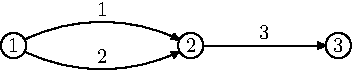
\includegraphics{p1-2-0}
\caption{习题1.2图}
\label{fig:p1-2}
\end{center}
\end{figure}
\end{exercise}

\begin{solution}
图示的交通网络中包含两条路径~:
\circlednum{1}$\xrightarrow{1}$\circlednum{2}$\xrightarrow{3}$\circlednum{3},
\circlednum{1}$\xrightarrow{2}$\circlednum{2}$\xrightarrow{3}$\circlednum{3}.
\par 设这两条路径上的旅行时间分别为~$t_1, t_2$, 三条路段上的交通流量分别为
~$x_1, x_2, x_3$, 根据~Wardrop~原理有
$$ \left\{\begin{aligned}
t_1 &= 2 + x_1^2\\
t_2 &= 1 + 3x_2\\
t_1 &= t_2\\
4 &= x_1 + x_2
\end{aligned}\right.
\Longrightarrow
\left\{\begin{aligned}
x_1^2 -3x_2 + 1 &= 0\\
x_1 + x_2 &= 4
\end{aligned}\right. $$
求解得到~$x_1 = \frac{\sqrt{53} - 3}{2}, x_2 = \frac{-\sqrt{53} + 11}{2}$, 节点处流量守恒有
~$x_3 = x_1 + x_2 = 4$. 均衡出行时间为~$t_1 = t_2 = \frac{-3\sqrt{53} + 35}{2}$
\end{solution}

\begin{exercise}
图~\ref{fig:p1-3}~所示网络中包含多条连接起点和终点的路段.每条路段的运行水平曲线都是线性的, 即是,
$$ t_a = A_a + B_ax_a $$
其中~$A_a$~和~$B_a$~为常数, 并且如习题~1.2~中所示,~$t_a$~和~$x_a$~分别表示路段~$a$~
上的旅行时间和交通流量. 起点和终点间的出行需求为~$q$~.
\begin{figure}[ht]
\begin{center}
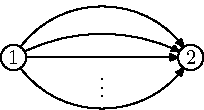
\includegraphics{p1-3-0}
\caption{习题1.3图}
\label{fig:p1-3}
\end{center}
\end{figure}
\begin{compactenum}[(1)]
\item 假设达到均衡时, 网络中所有的路段都有交通流量, 写出每个路段上流量的表达式.
\item 当在均衡状态不确定每个路段都被使用, 各个路段上的流量如何求解~(即只有部分路段被使用)?
\end{compactenum}
\end{exercise}

\begin{solution}
(1) 根据~Wardrop~条件, 达到均衡时各路段的交通量必须满足如下线性方程组
$$ \left\{ \begin{aligned}
t_i &= A_i + B_ix_i \quad i = 1,\ldots,n\\
t &= t_1 = t_2 = \ldots = t_n\\
q &= \sum_k x_k
\end{aligned} \right. $$
其中~$n$~为路段总数, $t$~为均衡时各路段的旅行时间. 各路段的流量为
$$ x_i = \frac{t_i - A_i}{B_i} = \frac{t - A_i}{B_i} \quad i\in[i,n]$$
将上式代入~$q = \sum_k x_k$~中
$$ q = \sum_k \frac{t - A_k}{B_k} = t\sum_k \frac{1}{B_k} - \sum_k \frac{A_k}{B_k} $$
于是均衡旅行时间为
$$ t = \frac{\sum_k \frac{A_k}{B_k} + q}{\sum_k \frac{1}{B_k}} $$
代入~$ x_i = \frac{t - A_i}{B_i}$~中就求得各路段的交通流量
$$ x_i = \frac{1}{B_i}\left[ \frac{\sum_k \frac{A_k}{B_k} + q}{\sum_k \frac{1}{B_k}} - A_i \right] $$
\par (2) 由第一问的结论可知路段~i~被使用应该满足如下条件
$$ x_i = \frac{1}{B_i}\left[ \frac{\sum_k \frac{A_k}{B_k} + q}{\sum_k \frac{1}{B_k}} - A_i \right] > 0 $$
即如果路段~i~被使用, 交通需求~$q$~应满足
$$ q > \sum_k \frac{A_i}{B_k} - \sum_k \frac{A_k}{B_k} $$
对于给定的~$q$, 可以根据上式确定已被使用的路段, 将未被使用的路段从交通网络中移除,
在剩余的网络中, 按照第一问做类似的求解即可.
\end{solution}

\section{最优化问题的基本概念}
在本章中, 作者提前预告了下一章需要用到的最优化理论和技巧, 为均衡配流的等价数学规划
问题的引入作准备.本章的一些习题是最优化理论中的重要定理~(如习题~2.1, 2.2, 2.3, 2.4),
它们的证明可以在一般的最优化理论教材中找到~(\cite{sundaram96}是作者喜欢的一本教材).
严格的说, 少数证明题的题设并不完善, 所以解题时我们认为题目中暗示了一些理所当然的条件.
从题目的选取可以察觉, 原书作者希望读者掌握最优化理论中的数学技巧, 理解直观的解释
~(如习题~2.11, 2.12, 2.17, 2.18).

\begin{exercise}%[(极小值的一阶必要条件)]
证明连续可导函数~$z(x)$~在极小值点处的一阶导数为零.
\end{exercise}

\begin{solution}
设函数~$z(x)$~在~$x^*$~处取极小值, 根据题设条件~$z(x)$~在~$x^*$~处可导, 所以对于任意的
数列~$y_k \rightarrow x^*$~有
$$ \lim_{k \rightarrow \infty} \frac{z(y_k) - z(x^*)}{y_k - x^*} = z'(x^*)$$
构造两个数列~${a_k}$~和~${b_k}$~分别满足条件~$a_k < x^* \ \forall k, a_k \rightarrow x^*$
和~$b_k > x^* \ \forall k, b_k \rightarrow x^*$. 因为在~$x^*$~处取得极小值, 所以存在领域
~$U(x^*, \epsilon)$, 使得对于足够大的~$k$~有~$z(a_k) \geq z(x^*),\, z(b_k) \leq z(x^*)$,于是
$$ \frac{z(a_k) - z(x^*)}{a_k - x^*} \geq 0 \geq \frac{z(b_k) - z(x^*)}{b_k - x^*} $$
当~$k \rightarrow \infty$~时, 对上式取极限有~$z'(x^*) \geq 0 \geq z'(x^*) $, 即~$z'(x^*) = 0$,
命题得证. 当~$z(\mathbf x)$~为多元函数时的证明可以参考\cite{sundaram96}.
\end{solution}

\begin{exercise}%[(凸函数的一阶充要条件)]
证明如果一个函数连续可微, 它是严格的凸函数当且仅当对该函数的线性近似总是低估其函数值.
(提示~: 证明如果条件~[2.4a]~成立, 那么条件~[2.4b]~也成立, 并且如果条件~[2.4b]~成立,
那么条件~[2.4a]~也成立.\footnote{原书中的公式~[2.4a]~和公式~[2.4b]~分别为
\begin{gather*}
z[\theta x_1 + (1 - \theta)x_2] < \theta z(x_1) + (1 - \theta)z(x_2)\\
z(x_1) + \frac{dz(x_1)}{dx}(x_2 - x_1)< z(x_2)
\end{gather*}})
\end{exercise}

\begin{solution}
首先证明必要性, 即已知公式~[2.4a]~证明公式~[2.4b].
任取函数定义域上的两点~$x_1,\,x_2$, 由函数连续可微有
$$ \frac{dz(x_1)}{dx}(x_2-x_1) = \lim_{\Delta x \rightarrow 0} \frac{z(x_1 + \Delta x) - z(x_1)}
{\Delta x} (x_2 - x_1)$$
取合适的~$t \in (0,1)$~使得~$\Delta x = t(x_2 - x_1)$, 于是
\begin{align*}
\lim_{\Delta x \rightarrow 0} \frac{z(x_1 + \Delta x) - z(x_1)}{\Delta x} (x_2 - x_1)
&= \lim_{t \rightarrow 0} \frac{z(x_1 + t(x_2 - x_1)) - z(x_1)}{t}\\
&= \lim_{t \rightarrow 0} \frac{z((1 - t)tx_1 + tx_2) - z(x_1)}{t}
\end{align*}
应用公式~[2.4a]~有~$z((1 - t)tx_1 + tx_2) - z(x_1) < tz(x_2) - tz(x_1)$于是
$$ \lim_{t \rightarrow 0} \frac{z((1 - t)tx_1 + tx_2) - z(x_1)}{t}
< \lim_{t \rightarrow 0} \frac{tz(x_2) - tz(x_1)}{t} = z(x_2) - z(x_1)$$
公式~[2.4b]~得证.
\par 再来证明充分性, 即已知公式~[2.4b]~证明公式~[2.4a].
任取函数定义域上的两点~$x_1,\,x_2$, 令~$x_{\theta} = \theta x_1 + (1 - \theta)x_2 \quad \theta \in (0,1)$,
应用公式~[2.4b]~有
\begin{align*}
z(x_2) - z(x_{\theta}) > \frac{dz(x_{\theta})}{dx}(x_2 - x_{\theta})
&= \frac{dz(x_{\theta})}{dx}(x_2 - x_1)\theta\\
z(x_1) - z(x_{\theta}) > \frac{dz(x_{\theta})}{dx}(x_1 - x_{\theta})
&= \frac{dz(x_{\theta})}{dx}(x_1 - x_2)(1 - \theta)
\end{align*}
上述不等式两边分别除以~$\theta, (1 - \theta)$~, 得到
\begin{align*}
\frac{1}{\theta}[z(x_2) - z(x_{\theta})] &> \frac{dz(x_{\theta})}{dx}(x_2 - x_1)\\
\frac{1}{(1 - \theta)}[z(x_1) - z(x_{\theta})] &> \frac{dz(x_{\theta})}{dx}(x_1 - x_2)
\end{align*}
将以上两式相加有
$$ \frac{1}{\theta}[z(x_2) - z(x_{\theta})] + \frac{1}{(1 - \theta)}[z(x_1) - z(x_{\theta})] > 0$$
整理得到
$$ z(x_{\theta}) < \theta(x_1) + (1 - \theta)(x_2) $$
公式~[2.4a]~得证. 当~$z(\mathbf x)$~为多元函数时可做类似的证明.
\end{solution}

\begin{exercise}%[(凸函数的二阶充要条件)]
证明如果一个函数二阶连续可导, 它是严格的凸函数当且仅当其二阶导数为正. (提示~: 证明如果
条件~[2.4a]~成立, 那么条件~[2.4c]~也成立, 并且如果条件~[2.4c]~成立,那么条件~[2.4a]~
也成立.\footnote{原书中的公式~[2.4c]~为 $$\frac{d^2z(x^*)}{dx^2} > 0$$})
\end{exercise}

\begin{solution}
首先证明必要性, 即由公式~[2.4a]~证明公式~[2.4c]. 为了简化证明过程, 根据习题~2.2~可以通过
公式~[2.4b]~证明公式~[2.4c]~成立.
任取函数定义域上的两点~$x_1,\,x_2\,(x_1 < x_2)$, 由公式~[2.4b]~分别有
\begin{align*}
\frac{dz(x_1)}{dx}(x_2 - x_1) &< z(x_2) - z(x_1)\\
\frac{dz(x_2)}{dx}(x_1 - x_2) &< z(x_1) - z(x_2)
\end{align*}
将上述两式均除以~$(x_2 - x_1)$
\begin{align*}
\frac{dz(x_1)}{dx} &< \frac{z(x_2) - z(x_1)}{x_2 - x_1}\\
-\frac{dz(x_2)}{dx} &< \frac{z(x_1) - z(x_2)}{x_2 - x_1}
\end{align*}
将两式相加得
$$ \frac{dz(x_1)}{dx} - \frac{dz(x_2)}{dx} < 0 $$
这个就证明了导函数~$\frac{dz(x)}{dx}$~单调递增, 显然其二阶导数满足
$$ \frac{d^2z(x)}{dx^2} > 0$$
\par 再来证明充分性, 即由公式~[2.4c]~证明公式~[2.4a]. 任取函数定义域上的两点~$x_1,\,x_2$,
令~$x_{\theta} = \theta x_1 + (1 - \theta)x_2 \quad \theta \in (0,1)$. 由函数二阶连续可导,
应用微分中值定理, 存在~$\omega_1 \in (x_1, x_{\theta}),\,\omega_2 \in (x_{\theta}, x_2)$~使得
\begin{align*}
\frac{z(x_{\theta}) - z(x_1)}{x_{\theta} - x_1} &= z'(\omega_1)\\
\frac{z(x_2) - z(\theta)}{x_2 - x_{\theta}} &= z'(\omega_2)
\end{align*}
由~$\omega_1 < \omega_2$~及函数的二阶条件~[2.4c]~有
$$ z'(\omega_1) < z'(\omega_2) $$
于是
$$ \frac{z(x_{\theta}) - z(x_1)}{x_{\theta} - x_1}
< \frac{z(x_2) - z(\theta)}{x_2 - x_{\theta}} $$
将~$x_{\theta} = \theta x_1 + (1 - \theta)x_2$~带入上式
$$ \frac{z(x_{\theta}) - z(x_1)}{(1 - \theta)(x_2 - x_1)}
< \frac{f(x_2) - z(\theta)}{\theta(x_2 - x_1)} $$
整理得
$$ z(x_{\theta}) < \theta z(x_1) + (1 - \theta)z(x_2) $$
公式~[2.4a]~得证. 当~$z(\mathbf x)$~为多元函数时的证明可以参考\cite{sundaram96}.
\end{solution}

\begin{exercise}
数学规划的~$\min z(\mathbf x)$~约束条件为~$g_j(\mathbf x) \geq b_j$, 其中~$j = 1,\ldots,J$,
该数学规划在下面那种情况有唯一的极小值? 回答问题并解释原因.
\begin{compactenum}[(a)]
\item 函数~$z(\mathbf x)$~是凸函数且约束集为凸.
\item 函数~$z(\mathbf x)$~有唯一的极小值且无约束.
\item 函数~$z(\mathbf x)$~单调递增且无约束.
\item 函数~$z(\mathbf x)$~是凹函数且约束集为凸.
\item 函数~$z(\mathbf x)$~在凸约束集中分段连续.
\end{compactenum}
\end{exercise}

\begin{solution}
该数学规划满足~(a)~时有唯一的极小值, 在证明中我们需要使用如下定理~(它们的证明可以参见~\cite{sundaram96}~):\\
如果~$D \subset \Re^n$~是凸集, 且~$f: D \rightarrow \Re$~是凸函数, 那么
\begin{compactenum}
\item 函数~$f$~的任何局部极小值都是全局最小值.
\item 函数~$f$~在~$D$~上的极值点的集合~$\arg \max \{f(\mathbf x)|\;\mathbf x \in D\}$~是空集或凸集.
\end{compactenum}
\par 现在证明本题的结论. 假设~$\arg \max \{z(\mathbf x)|\;\mathbf x \in D\}$~是非空集合,
我们需要证明它仅包含一个点.从上面的定理可知~$\arg \max \{z(\mathbf x)|\;\mathbf x \in D\}$~是凸集,
设函数有两个不同的极小值~$\mathbf x_1^*,\,\mathbf x_2^*$, 令~$\mathbf x_{\theta} = \theta
\mathbf x_1^* + (1 - \theta)\mathbf x_2^* \quad \theta \in (0,1)$. 显然~$\mathbf x_{\theta}
\in \arg \max \{z(\mathbf x)|\;\mathbf x \in D\}$~是函数的极值点, 所以有~$z(\mathbf x_{\theta}) =
z(\mathbf x_1^*) = z(\mathbf x_2^*)$.
但是由函数~$z(\mathbf x)$~的严格凸性有
\begin{align*}
z(\mathbf x_{\theta}) = z(\theta \mathbf x_1^* + (1 - \theta)\mathbf x_2^*)
> \theta z(\mathbf x_1^*) + (1 - \theta)z(\mathbf x_2^*) = z(\mathbf x_1^*)
\end{align*}
与先前的假设矛盾, 所以~$z(\mathbf x)$~在~$D$~上仅有一个极小值.
\end{solution}

\begin{exercise}
考虑数学规划~$\min z(x) = (x - 2)^2$, 约束条件为~$0 \leq x \leq 1$.
\begin{compactenum}[(a)]
\item 将上述数学规划写作标准形式.
\item 证明在可行域中~$z(x)$~的极小值点满足一阶条件~[2.7]%
\footnote{原书中的公式~[2.7]~为
\begin{gather*}
\frac{dz(x^*)}{dx} = \sum_j u_j \frac{dg_j(x^*)}{dx}\\
u_j \geq 0,\ u_j[b_j - g_j(x^*)] = 0,\ g_j(x^*) \geq b_j, \quad j = 1,\ldots,J
\end{gather*}}.
\end{compactenum}
\end{exercise}

\begin{solution}
(a) 写作标准形式~:
\begin{align*}
\min z(x) &= (x - 2)^2\\
s.t\ -x &\geq -1\\
x &\geq 0
\end{align*}
\par (b) 函数~$z(x)$~在区间~[0,1]~上单调递减, 极小值在~$x = 1$~处取得, 有
\begin{align*}
\left.\frac{dz(x)}{dx}\right|_{x = 1} &= 2(x - 2)|_{x = 1} = -2\\
\left.\frac{dg_1(x)}{dx}\right|_{x = 1} &= -1\\
\left.\frac{dg_2(x)}{dx}\right|_{x = 1} &= 1
\end{align*}
存在~$u_1 = 2,\,u_2 = 0$~满足一阶条件~[2.7].
\end{solution}

\begin{exercise}
绘制二维函数~$z(x_1,x_2)$~的等高线图~(仅绘制可行域范围), 约束条件为~$0 \leq x_1 \leq a$, $0 \leq x_2 \leq b$,
假设该函数有如下性质~:
\begin{compactenum}[(a)]
\item 是严格的凸函数.
\item 在多个最小值处为凸.
\item 是线性的.
\item 有约束条件~$x_1 + x_2 = c$~(外加前面的约束条件).
\end{compactenum}
\end{exercise}

\begin{solution}
(解答暂缺)
\end{solution}

\begin{exercise}
证明梯度总是指向函数~$z(\mathbf x)$~的最速上升方向~(局部).
\end{exercise}

\begin{solution}
在所有范数~$\|\mathbf d\| = 1$~的方向中, 最速上升方向为
$$ \overline{\mathbf d} = \frac{\nabla z(\mathbf x)}{\|\nabla z(\mathbf x)\|} $$
根据下边的不等式可以得到这个结论
$$ \nabla z(\mathbf x)^{T}\mathbf d \leq \|\nabla z(\mathbf x)\| \|\mathbf d\| =
\nabla z(x)^{T} \left( \frac{\nabla z(\mathbf x)}{\|\nabla z(\mathbf x) \|} \right) =
\nabla z(x)^{T} \overline{\mathbf d} $$
还可以根据下面的最大值问题来求得最速上升方向
\begin{gather*}
\max_{d} \nabla z(\mathbf x) \mathbf d\\
s.t.\quad \|\mathbf d\| = 1
\end{gather*}
运用拉格朗日定理求解有类似的结果.
\end{solution}

\begin{exercise}
计算函数~$z(x_1,x_2) = 2(x_1 - 3)^2 + 3(x_2 - 2)^2$~在点~$(x_1,x_2) = (2,3)$~
和~$(x_1,x_2) = (3,2)$~处的梯度.
\end{exercise}

\begin{solution}
函数~$z(x)$~的梯度为
$$ \nabla z(x_1,x_2) =
\begin{pmatrix}
4(x_1 - 3) \\
6(x_2 - 2)
\end{pmatrix} $$
点~$(x_1,x_2) = (2,3)$~和~$(x_1,x_2) = (3,2)$~处的梯度
\begin{align*}
\nabla z(x_1,x_2)|_{(x_1,x_2) = (2,3)} &=
\begin{pmatrix}
-4 \\ 6
\end{pmatrix}\\
\nabla z(x_1,x_2)|_{(x_1,x_2) = (3,2)} &=
\begin{pmatrix}
0 \\ 0
\end{pmatrix}
\end{align*}
\end{solution}

\begin{exercise}
证明凸函数的和组成的函数也是凸函数.
\end{exercise}

\begin{solution}
首先证明两个凸函数的和组成的函数是凸函数. 设两个凸函数分别为~$f: D_1 \rightarrow \Re$~和
~$g: D_2 \rightarrow \Re$, 它们的定义域分别为~$D_1 \subset \Re^n$~和~$D_2 \subset \Re^n$,
且都是凸集. 两函数和组成的函数为~$h: D_3 \rightarrow \Re$, 其中~$D_3 = D_1 \cap D_2$.
现在证明函数~$h(x)$~是凸函数. 任取两个点~$x_1,\,x_2 \in D_3\; (x_1 \neq x_2)$, 且令
~$x_{\theta} = \theta x_1 + (1 - \theta)x_2,\ \theta \in (0,1)$~
\begin{align*}
h(x_{\theta}) &= h(\theta x_1 + (1 - \theta)x_2)\\
&= f(\theta x_1 + (1 - \theta)x_2) + g(\theta x_1 + (1 - \theta)x_2)\\
&> \theta f(x_1) + (1 - \theta)f(x_2) + \theta g(x_1) + (1 - \theta)g(x_2)\\
&= \theta [f(x_1) + g(x_1)] + (1 - \theta)[f(x_2) + g(x_2)]\\
&= \theta h(x_1) + (1 - \theta)h(x_2)
\end{align*}
于是证明了~$h(x)$~是凸函数. 多个凸函数的和组成的函数的凸性可以在此基础上证明.
\end{solution}

\begin{exercise}
求解数学规划~[2.15]\footnote{原书中数学规划~[2.15]~为
\begin{gather*}
\min z(x_1,x_2) = x_1^2 + 2x_2^2 + 2x_1x_2 - 2x_1 - 4x_2\\
\text{s.t.}\ x_1 + x_2 \geq 2
\end{gather*}}%
得到对偶变量的值为~$u^* = 2$. 稍微松驰约束条件, 再次进行求解.
验证~$u^*$~衡量了~$z(\mathbf x^*)$~对约束条件的灵敏度.
\end{exercise}

\begin{solution}
该数学规划对应的拉格朗日函数为
$$ L(x_1,x_2,u) = z(x_1,x_2) - u(x_1 + x_2 -2) $$
根据~Kuhn-Tucker~条件有
\begin{gather*}
\begin{aligned}
\frac{\partial L}{\partial x_1} &= 2x_1 + 2x_2 - 2 - u = 0\\
\frac{\partial L}{\partial x_2} &= 2x_1 + 4x_2 - 4 - u = 0\\
u\frac{\partial L}{\partial u} &= u(2 - x_1 - x_2) = 0
\end{aligned}\\
x_1 + x_2 \geq 2\\
u \geq 0
\end{gather*}
求方程组得~$u = 2,\;x_1 = 1,\;x_2 = 1$, 函数值为~$z(x_1,x_2) = -1$. 稍微松驰约束条件
$$ x_1 + x_2 \geq 2.1 $$
根据~Kuhn-Tucker~条件再次求解
\begin{gather*}
\begin{aligned}
\frac{\partial L}{\partial x_1} &= 2x_1 + 2x_2 - 2 - u = 0\\
\frac{\partial L}{\partial x_2} &= 2x_1 + 4x_2 - 4 - u = 0\\
u\frac{\partial L}{\partial u} &= u(2.1 - x_1 - x_2) = 0
\end{aligned}\\
u \geq 0, \quad x_1 + x_2 \geq 2.1
\end{gather*}
解得~$u = 2.1,\;x_1 = 1.15,\;x_2 = 0.95$, 函数值为~$z(x_1,x_2) = -0.7875$. 函数值的变化为
~$\nabla z(x_1,x_2) = 0.2125 $, 近似于~$u\Delta b = 0.2$.
\end{solution}

\begin{exercise}
\begin{compactenum}[(a)]
\item 运用~Kuhn-Tucker~条件, 证明如果仅有非负约束则公式~[2.19]%
\footnote{原书中的公式~[2.19]~为 $$x_i^*\frac{\partial z(\mathbf x^*)}{\partial x_i} = 0
~\text{且}~\frac{\partial z(\mathbf x^*)}{\partial x_i} \geq 0~\text{其中}~i = 1,2,\ldots,I$$}成立.
\item 直接从~Kuhn-Tcker~条件~(公式~[2.14]\footnote{原书中的公式~[2.14]~为
\begin{gather*}
\frac{\partial z(\mathbf x^*)}{\partial x_i} = \sum_j u_j \frac{\partial g_i(\mathbf x^*)}{\partial x}\\
u_j \geq 0,\ u_j[b_j - g_j(\mathbf x^*)] = 0,\ g_j(\mathbf x^*) \geq b_j,\ \text{其中}~j = 1,\ldots,J
\end{gather*}})~%
推导出公式~[2.28]\footnote{原书中的公式~[2.28]~为
\begin{align*}
x_i^* \left( \frac{\partial z(\mathbf x^*)}{\partial x_i} - \sum_j u_j^*h_{ij} \right) &= 0\ \forall i \\
\frac{\partial z(\mathbf x^*)}{\partial x_i} - \sum_j u_j^*h_{ij} &\geq 0\ \forall i \\
\sum_i h_{ij}x_i^* &= b_j\ \forall j \\
x_i^* &\geq 0\ \forall i
\end{align*}}.
\end{compactenum}
\end{exercise}

\begin{solution}
(a)~如果仅有非负约束则数学规划的标准形式如下
\begin{gather*}
\min z(\mathbf x)\\
s.t.\quad \mathbf x \geq 0
\end{gather*}
运用~Kuhn-Tucker~条件有
\begin{align*}
\nabla z(\mathbf x) - \mathbf u &= 0\\
\mathbf x^T \mathbf u &= 0\\
\mathbf x \geq 0,\ \mathbf u &\geq 0
\end{align*}
将~$\mathbf u = \nabla z(\mathbf x)$~分别代入~$\mathbf x^T \mathbf u = 0$~和~$\mathbf u \geq 0$
\begin{align*}
\mathbf x^T \nabla z(\mathbf x) &= 0\\
\nabla z(\mathbf x) &\geq 0
\end{align*}
于是公式~[2.19]~成立.
\par (b)~按照上面的方法做类似推导可以得到~公式~[2.28].
\end{solution}

\begin{exercise}[(灵敏度分析)]%
函数~$z(\mathbf x)$~的约束条件为~$g_j(\mathbf x) \geq b_j$, 其中~$j = 1,\ldots J$,
运用其拉格朗日函数解释为什么第~$j$~个约束条件稍微松驰~$\Delta b_j$, 将使目标函数%
~$z(\mathbf x)$~减小~$u_j\Delta b_j$.
\end{exercise}

\begin{solution}
假设最优解~$\mathbf x^*$~是约束条件中向量~$\mathbf b$~的函数, 并且连续可导, 那么有
$$ y(\mathbf b) = z(\mathbf x^*(\mathbf b))$$
即将目标函数写成关于~$\mathbf b$~的函数的形式, 对它求偏导数有
$$ \partialfrac{y}{b_i} = \sum_j \partialfrac{z}{x_j} \cdot \partialfrac{x^*_i}{b_i}$$
设~$h(\mathbf x) = g(\mathbf x) - \mathbf b$, 原目标函数关于~$x_i$~的偏导数为
$$ \partialfrac{z}{x_j} = \sum_k u_k \cdot \partialfrac{h_k}{x_j}$$
将上式代入~$\partialfrac{y}{b_i}$~中有
\begin{equation*} \begin{split}
\partialfrac{y}{b_i} &= \sum_j \left(\sum_k u_k \cdot \partialfrac{h_k}{x_j}\right) \cdot \partialfrac{x^*_j}{b_i}\\
&= \sum_k u_k \cdot \sum_j \partialfrac{h_k}{x_j} \cdot \partialfrac{x^*_j}{b_i}\\
\end{split} \end{equation*}
因为~$\partialfrac{g_k}{x_j} = \partialfrac{h_j}{x_l}$~所以
$$ \partialfrac{h_k}{b_i} = \left\{
\begin{aligned}
&\partialfrac{g_k}{b_i} - 1 = \sum_j \partialfrac{h_k}{x_j} \cdot \partialfrac{x_j}{b_i} - 1 &k = i\\
&\partialfrac{g_k}{b_i} = \sum_j \partialfrac{h_k}{x_j} \cdot \partialfrac{x_j}{b_i} &k \neq i
\end{aligned} \right. $$
于是有
$$ \partialfrac{y}{b_i} = u_i$$
所以第~$j$~个约束条件稍微松驰~$\Delta b_j$, 将使目标函数~$z(\mathbf x)$~减小~$u_j\Delta b_j$.
\end{solution}

\begin{exercise}
运用~Kuhn-Tucker~条件, 求解数学规划
\begin{align*}
\min z(x_1,x_2) = 4(x_1 &- 2)^2 + 3(x_2 - 4)^2\\
\text{s.t.}\
x_1 + x_2 &\geq 5\\
x_1 &\geq 1\\
x_2 &\geq 2
\end{align*}
证明解是唯一的.
\end{exercise}

\begin{solution}
目标函数的~Hessian~矩阵为
$$ \nabla^2 z(x_1,x_2) = \begin{pmatrix} 8 & 0\\0 & 6 \end{pmatrix} $$
并且可行域是一个凸集, 所以该数学规划有唯一的极小值. 运用~Kuhn-Tucker~条件容易求得
$(x_1, x_2) = (2, 4)$~时有最小值~$z(x_1, x_2) = 0$.
\end{solution}

\begin{exercise}
运用拉格朗日函数, 求解数学规划
\begin{align*}
\min z(x_1,x_2) = 5x_1^2 &- 3x_1x_2 + 2x_2^2 +7\\
\text{s.t.}\ 2x_1 + x_2 &= 5\\
x_1 &\geq 0\\
x_2 &\geq 0
\end{align*}
画出可行域.
\end{exercise}

\begin{solution}
由目标函数和等式约束条件得到拉格朗日函数
$$ L(x_1,x_2,\lambda) = 5x_1^2 - 3x_1x_2 + 2x_2^2 +7 + \lambda (2x_1 + x_2 - 5)$$
求解下面的方程组
$$ \left\{ \begin{aligned}
x_1 \partialfrac{L}{x_1} &= 0\\
x_2 \partialfrac{L}{x_2} &= 0\\
\partialfrac{L}{\lambda} &= 0
\end{aligned} \right. $$
满足约束的解为~$x_1 = \frac{55}{38}, x_2 = \frac{80}{38}$, 函数最小值为~$z(x_1, x_2) = \frac{1307}{76}$.
\end{solution}

\begin{exercise}
求解数学规划
\begin{align*}
\min z(x_1,x_2) = 2x_1 &+ x_2\\
\text{s.t.}\ 3x_1 + x_2 &\geq 1\\
x_1 + 4x_2 &\geq 2\\
-x_1 + x_2 &\geq 1
\end{align*}
画出可行域及目标函数的等高线图.
\end{exercise}

\begin{solution}
根据~Kuhn-Tucker~条件如下方程组成立
$$ \left\{ \begin{aligned}
2 - 3u_1 -u_2 +u_3 &= 0\\
1 - u_1 - 4u_2 - u_3 &= 0\\
u_1(3x_1 + x_2 - 1) &= 0\\
u_2(x_1 + 4x_2 - 2) &= 0\\
u_3(-x_1 + x_2 - 1) &= 0
\end{aligned} \right. $$
满足约束条件的解为~$x_1 = 0, x_2 = 1$, 函数最小值为~$z(x_1, x_2) = 1$.
\end{solution}

\begin{exercise}
给定函数
$$z(x_1,x_2,x_3) = 3x_1^2 + 2x_1x_2 + 6x_2^2 - x_2x_3 + 5x_3^2 - 4x_1 - 2x_2 - 6x_3 +9$$
\begin{compactenum}[(a)]
\item 计算~$z(x_1,x_2,x_3)$~的极小值.
\item 验证这是局部极小值.
\item 验证这个局部极小值是全局最小值.
\end{compactenum}
\end{exercise}

\begin{solution}
首先, 解下面的方程组得到函数的驻点
$$ \left\{ \begin{aligned}
\partialfrac{z}{x_1} &= 0\\
\partialfrac{z}{x_2} &= 0\\
\partialfrac{z}{x_3} &= 0
\end{aligned} \right. $$
解得~$x_1 = \frac{212}{337}, x_2 = \frac{38}{337}, x_3 = \frac{206}{337}, z(x_1, x_2, x_3) = \frac{1953}{337}$.
函数的~Hessian~矩阵为
$$ \nabla^2 z(x_1, x_2, x_3) =
\begin{pmatrix}
6 & 2 & 0\\
2 & 12 & -1\\
0 & -1 & 10
\end{pmatrix} $$
容易验证上述矩阵是正定的, 所以求得的局部最小值是全局最小值.
\end{solution}

\begin{exercise}
如果对偶变量表示目标函数值得改进, 联系约束条件的松驰, 解释为什么对有标准不等式约束的
极小值问题有~$u_j \geq 0, \forall j$, 而在等式约束中~$u_j$~能取任意的符号.
\end{exercise}

\begin{solution}
下面的求解仅仅是一种直观的解释, 严格的证明可以参见~\cite{sundaram96}. 原书中标准的极小值问题有如下形式
\begin{gather*}
\min z(\mathbf x)\\
s.t. \quad g_j(\mathbf x) \geq b_j, \quad j = 1,\ldots, J
\end{gather*}
若上述极小值问题达到极小值时有~$g_j(\mathbf x) > b_j$, 松驰这一约束条件并不会帮助减小函数值,
所以有~$u_j = 0$. 当~$g_j(\mathbf x) = b_j$~时, 根据习题~2.12, 知道~$b_j$~稍微减小~$\Delta b_j$,
将使目标函数~$z(\mathbf x)$~减小~$u_j\Delta b_j$, 于是有~$u_j \geq 0$.
\par 在等式约束中, 总是有~$g_j(\mathbf x) = b_j$, 增加或减小~$b_j$~都有可能减小目标函数的值,
所以~$u_j$~的符号并不确定.
\end{solution}

\begin{exercise}
不使用拉格朗日函数写出下面数学规划的~Kuhn-Tucker~条件~(提示~: 将约束条件写作标准形式.)
\begin{gather*}
\min z(\mathbf x)\\
\text{s.t.}\ \sum_i h_{ij}x_i = b_j \ \forall j
\end{gather*}
证明等式约束的对偶变量可取任意符号.
\end{exercise}

\begin{solution}
如题目中提示的, 将数学规划写作标准形式
\begin{gather*}
\min z(\mathbf x)\\
s.t.\quad
\begin{aligned}
\sum_i h_{ij}x_i &\geq b_j\\
-\sum_i h_{ij}x_i &\geq -b_j
\end{aligned}
\quad \forall  j
\end{gather*}
上述数学规划的~Kuhn-Tucker~条件为
\begin{align*}
\begin{aligned}
\partialfrac{z}{x_i} - \sum_j u_j h_{ij} &= 0\\
\partialfrac{z}{x_i} + \sum_j \lambda_j h_{ij} &= 0
\end{aligned} \quad &\forall i\\
\begin{aligned}
u_j(\sum_i h_{ij}x_i - b_j) &= 0\\
\lambda_j(-\sum_i h_{ij}x_i + b_j) &= 0\\
u_j \geq 0, \lambda_j &\geq 0
\end{aligned} \quad &\forall j
\end{align*}
其中~$u_j, \lambda_j$~为对偶变量. 我们将前四个式子两两相加
\begin{align*}
\partialfrac{z}{x_i} - \sum_j (u_j - \lambda_j)h_{ij} = 0 \quad &\forall i\\
\begin{aligned}
(u_j - \lambda_j)(\sum_i h_{ij}x_i - b_j) &= 0\\
u_j \geq 0, \lambda_j &\geq 0
\end{aligned} \quad &\forall j
\end{align*}
将式中的~$u_j - \lambda_j$~替换为~$\theta_j$, 显然新的对偶变量~$\theta_j$~的符号没有限制.
\end{solution}

\section{交通分配的数学规划模型}
本章的第~1~节给出了~Wardrop~原理的数学规划模型; 第~2, 3~节根据上一章的预备知识证明了
该模型的正确性, 并讨论解的唯一性需要满足的条件. 第~4, 5~节介绍了系统最优原理的数学
规划模型, 以及它与用户均衡配流的关系. 本章的习题要求读者运用非线性规划理论解释交通
分配问题, 引导读者探究借助~Kuhn-Tucker~条件转换~Wardrop~原理的精巧之处.

\begin{exercise}
考虑图~\ref{fig:p3-1}~中的网络. 它包含了两个~O--D~对~(1 $\rightarrow$ 4~和~2 $\rightarrow$ 4)
和五条路段~(路段的编号标在各路段上). 将各路径编号并且指出每条路径的走向. 写出这个网络
的路径--路段关联矩阵. 使用这个矩阵由~$\mathbf f$~得出~$x_3$.
\begin{figure}[ht]
\begin{center}
\includegraphics{p3-1-0};
\caption{习题~3.1~图}
\label{fig:p3-1}
\end{center}
\end{figure}
\end{exercise}

\begin{solution}
各路径的编号如下~:\\
路径~1: \circlednum{1} $\xrightarrow{4}$ \circlednum{4}\\
路径~2: \circlednum{1} $\xrightarrow{1}$ \circlednum{3} $\xrightarrow{3}$ \circlednum{4}\\
路径~3: \circlednum{2} $\xrightarrow{2}$ \circlednum{3} $\xrightarrow{3}$ \circlednum{4}\\
路径~4: \circlednum{2} $\xrightarrow{5}$ \circlednum{4}\\
于是~$\mathbf f = (f_1, f_2, f_3, f_4)$, 可以得到如下路段--路径关联矩阵
$$ \bordermatrix{%
  & 1 & 2 & 3 & 4 \cr
1 & 0 & 1 & 0 & 0 \cr
2 & 0 & 0 & 1 & 0 \cr
3 & 0 & 1 & 1 & 0 \cr
4 & 1 & 0 & 0 & 0 \cr
5 & 0 & 0 & 0 & 1
} $$
第~3~条路段上的流量为
$$ x_3 = \mathbf f \cdot (0, 1, 1, 0)^T = f_2 + f_4 $$
\end{solution}

\begin{exercise}
通过设置等价极小值问题和使用拉格朗日乘数法来求解图~\ref{fig:p3-2}~所示网络
\footnote{此图在原书的~62~页, O--D~对间的交通需求为~5, 两个路段的服务水平函数分别为~
$t_1 = 2 + x_1, t_2 = 1 + 2x_2$.}.
解释取得最优解时拉格朗日乘数的意义.
\begin{figure}[ht]
\begin{center}
\includegraphics{p3-2-0}
\caption{习题~3.2~图}
\label{fig:p3-2}
\end{center}
\end{figure}
\end{exercise}

\begin{solution}
对应的等价极小值问题为
\begin{gather*}
\min \int_0^{x_1} t_1(w)dw + \int_0^{x_2} t_2(w)dw\\
\begin{aligned}
s.t \quad x_1 + x_2 &= 5\\
x_1, x_2 &\geq 0
\end{aligned}
\end{gather*}
对应的拉格朗日函数为
$$ L(\mathbf x_1, x_2, u) = \int_0^{x_1} t_1(w)dw + \int_0^{x_2} t_2(x)dw + u(q - x_1 - x_2) $$
达到最优解时满足如下条件\footnote{通过~Kuhn-Tucker~条件求解函数极值的标准步骤是~:\\
1) 确定函数的最大值或最小值存在~(Weierstrass 定理),\\
2) 判别约束条件是否满足要求~(Constraint Qualitication),\\
3) 求解~Kuhn-Tucker~方程组, \\
4) 确定最优解.\\
由于等价数学规划的性质~(目标函数为凸和线性的约束条件), 解集中所有的求解过程略去步骤~1, 2~
(不影响结果的正确性). 这样做的理由请参阅~\cite{bertsekas99, sundaram96}.}
$$ \left\{
\begin{aligned}
\partialfrac{L}{x_1} &= 2 + x_1 - u = 0\\
\partialfrac{L}{x_2} &= 1 + 2x_2 - u = 0\\
\partialfrac{L}{u} &= 5 - x_1 -x_2 = 0
\end{aligned}
\right.$$
解得~$ x_1 = 3, x_2 = 2, u = 5$. 所以在最优解处, 拉格朗日乘数~$u$~等于每个路段当前的
服务水平, 也就是再增加一个单位的交通流所产生的行驶时间.
\end{solution}

\begin{exercise}
求解图~\ref{fig:p3-3}~中交通网络的用户均衡配流, 以及行驶时间, 其中
\begin{align*}
t_1 &= 2 + x_1^2\\
t_2 &= 3 + x_2\\
t_3 &= 1 + 2x_3^2\\
t_4 &= 2 + 4x_4
\end{align*}
(路段编号标注在各路段之上). 节点~1, 3~间有~4~单位的交通流量.
\begin{figure}[ht]
\begin{center}
\includegraphics{p3-3-0}
\caption{习题~3.3~图}
\label{fig:p3-3}
\end{center}
\end{figure}
\end{exercise}

\begin{solution}
对应的等价极小值问题为
\begin{gather*}
\min \sum_{i = 1}^4 \int_0^{x_i} t_i(w)dw\\
\begin{aligned}
s.t \quad &x_1 + x_2 = 4\\
&x_3 + x_4 = 4\\
&x_1, x_2, x_3, x_4 \geq 0
\end{aligned}
\end{gather*}
最优解应当满足如下方程组
$$ \left\{
\begin{aligned}
x_1(2 + x_1^2 - u_1) &= 0\\
x_2(3 + x_2 - u_1) &= 0\\
x_3(1 + 2x_3^2 - u_2) &= 0\\
x_4(2 + 4x_4 - u_2) &= 0\\
x_1 + x_2 &= 4\\
x_3 + x_4 &= 4\\
\end{aligned}
\right. $$
上述方程的解需要满足如下不等式组
$$ \left\{
\begin{aligned}
2 + x_1^2 - u_1 &\geq 0\\
3 + x_2 - u_1 &\geq 0\\
1 + 2x_3^2 - u_2 &\geq 0\\
2 + 4x_4 - u_2 &\geq 0\\
x_1, x_2, x_3, x_4 &\geq 0
\end{aligned}
\right. $$
满足上述条件的有多组解, 通过代入目标函数比较大小, 求得最优解
\footnote{这里给出的答案是习题解答集作者借助~Maple~的非线性方程求解功能得到的.}
\begin{gather*}
x_1 = 1.791287847, x_2 = 2.208712153\\
x_3 = 2.082207001, x_4 = 1.917792999\\
u_1 = 5.208712153, u_2 = 9.671171996
\end{gather*}
各路段的服务水平近似为
$$ t_1 = 5.2087, t_2 = 5.2087, t_3 = 9.6712, t_4 = 9.6712 $$
此时从节点~1~到节点~3~的行驶时间为~14.8799~个单位.
\par 本题为了计算上的简便, 没有使用原书中的关于路径流量的公式~[3.16]~进行计算\footnote{%
原书中的公式~[3.16]
\begin{align*}
f_k^{rs}(c_k^{rs} - u_{rs}) &= 0 \quad \forall k, r, s\\
c_k^{rs} - u_{rs} &\geq 0 \quad \forall k, r, s\\
\sum_k f_k^{rs} &= q \quad \forall k, r\\
f_k^rs &\geq 0 \quad \forall k, r, s
\end{align*}},
而是使用关于路段流量的方程组来求得最优解\footnote{实际上这是两种不同的网络表达形式,
有的文献称它们为~node--link~和~link-route. 感兴趣的读者可以参阅~\cite{patrksson94}
中的~2.2.2~小节以及经典教材~\cite{ahuja93}, 必须承认习题解答集作者对这个问题只是一知半解.}.
但是本题的计算量仍然很大, 方程组中前~4~个方程的求解需要试举~16~种不同的情况.
一般的, 如果交通网络中有~n~条路段, 可能需要进行~$2^n$~试举, 显然这样做的效率
是极低的, 所以高效的求解算法势在必行.
\end{solution}

\begin{exercise}
求解如图~\ref{fig:p3-4}~所示交通网络的均衡交通分配
\footnote{此图在原书的~68~页, 各路段的服务水平函数分别为
$$t_1 = 1,\;t_2 = 2,\;t_3 = 2 + x_3,\;t_4 = 1 + 2x_4,\;t_5 = 1$$
O--D~对间的交通需求分别为~$q_{15} = 2, q_{25} = 3$.}.
写出用户均衡的等价数学规划, 并且求解其一阶条件.
\begin{figure}[ht]
\begin{center}
\includegraphics{p3-4-0}
\caption{习题~3.4~图}
\label{fig:p3-4}
\end{center}
\end{figure}
\end{exercise}

\begin{solution}
写出等价的极小值问题
\begin{gather*}
\min \sum_i \int_0^{x_i} t_i(w)dw\\
s.t \quad x_1 = 2,\;x_2 = 3,\;x_3 + x_4 = 5,\;x_5 = 5\\
x_1, \ldots x_5, \geq 0
\end{gather*}
达到极小值时路段流量应该满足如下方程组
$$ \left\{
\begin{aligned}
x_1(1 - u_1) &= 0\\
x_2(2 - u_2) &= 0\\
x_3(2 + x_3 - u_3) &= 0\\
x_4(1 + 2x_4 - u_3) &= 0\\
x_5(1 - u_4) &= 0\\
x_1 = 2\quad x_2 &= 3\\
x_3 + x_4 = 5\quad x_5 &= 5
\end{aligned}
\right. $$
解得~$x_1 = 2, x_2 = 3, x_3 = 2, x_4 = 3, x_5 = 5$. 细心的读者可以发现本题中
节点~3~到节点~4~的一段网络是习题~3.2~的翻版.
\end{solution}

\begin{exercise}
\begin{compactenum}[(a)]
\item 将如图~\ref{fig:p3-4}~所示网络对应的用户均衡目标函数的~Hessian~矩阵用路径
流量表示出来. 确定这个矩阵是非正定的.
\item 证实用路径流量表示的用户均衡目标函数的~Hessian~矩阵, 在通常情况下不是正定
矩阵. 对于何种类型的交通网络这个~Hessian~矩阵是正定的?
\end{compactenum}
\end{exercise}

\begin{solution}
(a) 目标函数的二阶偏导数有如下形式
$$ \frac{\partial^2 z(\mathbf f)}{\partial f_m^{ab} \partial f_n^{cd}}
= \ldots + \frac{t_i(x_i)}{dx_i} + \ldots$$
上式等号右边的是一些路段服务水平函数的导函数, 经过一些尝试可以发现~: 如若导函数
~$\frac{t_i(x_i)}{dx_i}$~在式中出现, 那么路段~i~必是路径~$f_m^{ab}$~和路径~$f_n^{cd}$
都经过的. 根据这一规律足以给出本小题的解答
$$ \nabla^2 z(\mathbf f) =
\begin{pmatrix}
1 & 0 & 1 & 1\\
0 & 2 & 0 & 2\\
1 & 0 & 1 & 1\\
1 & 2 & 1 & 3
\end{pmatrix} $$
上述~Hessian~矩阵的行列式的值为零, 显然不是正定矩阵.
\par (b) 回答第~2~小问必须知道~Hessian~矩阵的闭合形式, 实际上是将它写做一些矩阵
运算的结果. 再结合第~1~小问中得到的规律, 不难发现
$$ \nabla^ 2 z(\mathbf f) = \Delta^T \cdot diag\left[\frac{t_1(x_1)}{dx_1}, \frac{t_2(x_2)}{dx_2},
\ldots, \frac{t_n(x_n)}{dx_n}\right] \cdot \Delta$$
其中~$\Delta$~为路段--路径关联矩阵, ~$diag[\ldots]$~是由导函数组成的对角矩阵.
\par 现在要讨论的是~: 在什么情况下目标函数的~Hessian~矩阵是正定的. 根据正定矩阵的定义,
如果~$\nabla^2 z(\mathbf f)$~是正定矩阵, 那么有
$$ \mathbf y^T \cdot \nabla^2 z(\mathbf f) \cdot \mathbf y > 0\quad \forall \mathbf y$$
即 $$ (\Delta \cdot \mathbf y)^T \cdot diag\left[\frac{t_1(x_1)}{dx_1}, \frac{t_2(x_2)}{dx_2},
\ldots, \frac{t_n(x_n)}{dx_n}\right] \cdot (\Delta \cdot \mathbf y) > 0 \quad \forall \mathbf y$$
如果各路段的服务水平函数均单调递增, 则对角矩阵~$diag\left[\frac{t_1(x_1)}{dx_1}, \frac{t_2(x_2)}{dx_2},
\ldots, \frac{t_n(x_n)}{dx_n}\right]$~为正定矩阵, 于是上面的不等式成立.
\end{solution}

\begin{exercise}
证明一个单调增函数的积分函数是凸函数.
\end{exercise}

\begin{solution}
我们只需证明该积分函数的二阶导数为正, 即证明原函数的导函数为正, 而题设中已知
原函数单调递增, 那么该积分函数是凸函数无疑.
\end{solution}

\begin{exercise}
求解如图~\ref{fig:p3-2}~所示网络的系统最优配流. 将该交通流形态与用户均衡配流的
交通流形态进行比较, 并且解释他们的差异.
\end{exercise}

\begin{solution}
系统最优配流的数学规划为
\begin{gather*}
\min t_1(x_1) x_1 + t_2(x_2) x_2\\
\begin{aligned}
s.t. \quad x_1 + x_2 &= 5\\
x_1, x_2 &\geq 0
\end{aligned}
\end{gather*}
对应的拉格朗日函数为
$$ L(x_1, x_2, u) = (2+x_1)x_1 + (1 + 2x_2)x_2 + u(5 - x_1 - x_2) $$
达到最优解时满足如下条件
$$ \left\{
\begin{aligned}
\partialfrac{L}{x_1} = 2 + 2x_1 - u &= 0\\
\partialfrac{L}{x_2} = 1 + 4x_2 - u &= 0\\
\partialfrac{L}{u} = 5 - x_1 - x_2 &= 0
\end{aligned}
\right. $$
解得~$x_1 = \frac{19}{6}, x_2 = \frac{11}{6}$, 习题~3.2~交通分配情况为~$x_1 = 3, x_2 = 2$.
对比用户均衡配流, 在系统最优配流中, 路段~1~的流量增加了~$\frac{1}{6}$~个单位.
\end{solution}

\begin{exercise}
求解习题~3.3~中交通网络的系统最优配流. 将它和用户均衡配流的结果进行比较.
\end{exercise}

\begin{solution}
系统最优配流的数学规划为
\begin{gather*}
\min \sum_{i = 1}^4 t_i(x_i)x_i\\
\begin{aligned}
s.t \quad &x_1 + x_2 = 4\\
&x_3 + x_4 = 4\\
&x_1, x_2, x_3, x_4 \geq 0
\end{aligned}
\end{gather*}
最优解满足如下方程组
$$ \left\{
\begin{aligned}
x_1(2 + 3x_1^2 - u_1) &= 0\\
x_2(3 + 2x_2 - u_1) &= 0\\
x_3(1 + 6x_3^2 - u_2) &= 0\\
x_4(2 + 8x_4 - u_2) &= 0\\
x_1 + x_2 &= 4\\
x_3 + x_4 &= 4
\end{aligned}
\right. $$
上述方程的解还需要满足如下不等式组
$$ \left\{
\begin{aligned}
2 + 3x_1^2 - u_1 &\geq 0\\
3 + 2x_2 - u_1 &\geq 0\\
1 + 6x_3^2 - u_2 &\geq 0\\
2 + 8x_4 - u_2 &\geq 0\\
x_1, x_2, x_3, x_4 &\geq 0
\end{aligned}
\right. $$
满足上述条件的有多组解, 通过代入目标函数比较大小, 求得最优解
\footnote{与习题~3.3~一样, 这里的结果也是用~Maple~求得的.}
\begin{gather*}
x_1 = 1.430500874, x_2 = 2.569499126\\
x_3 = 1.771456473, x_4 = 2.228543527\\
u_1 = 8.138998252, u_2 = 19.82834822
\end{gather*}
各路段的服务水平近似为
$$ t_1 = 4.0463, t_2 = 5.5695, t_3 = 7.2761, t_4 = 10.9142 $$
目标为函数值~$57.3111$.
\end{solution}

\begin{exercise}
就路径流量而言, 系统最优配流的数学规划是否有唯一解? 解释你的回答.
\end{exercise}

\begin{solution}
这里所说的唯一解是指目标函数有唯一的极小值点, 也就是要求目标函数为凸函数. 从习题~3.5~我们
得到提示~: 判别目标函数的~Hessian~矩阵是否正定. 根据原书中的公式~[3.24], 目标函数的~Hessian
矩阵为
$$ \nabla^ 2 z(\mathbf f) = \Delta^T \cdot
diag\left[\ldots, 2\frac{dt_i(x_i)}{dx_i} + x_i\frac{d^2t_i(x_i)}{dx_i^2}, \ldots \right] \cdot \Delta$$
于是问题再次归结为判别对角矩阵~$diag\left[\ldots, 2\frac{dt_i(x_i)}{dx_i} + x_i\frac{d^2t_i(x_i)}{dx_i^2},
\ldots \right]$~的正定性. 如果我们做更强的假设~: 路段服务水平函数单调递增且是凸函数, 则系统最优配流有唯一解.
\end{solution}

\begin{exercise}
\begin{compactenum}[(a)]
\item 证明路段行驶时间为~$\hat{\hat{t}}_a(x_a)$~(参见公式~[3.29]\footnote{原书中的公式~[3.29]
$$ \hat{\hat{t}}_a(x_a) = \frac{1}{x_a} \int_0^{x_a} t_a(w)dw $$ })
的系统最优配流解是用户均衡配流.
\item 证明路段行驶时间为~$\tilde{r}_a(x_a)$~(参见公式~[3.24]\footnote{原书中的公式~[3.24]
$$\tilde{t}_a(x_a) = t_a(x_a) + x_a \frac{dt_a(x_a)}{dx_a}$$})
的用户均衡配流解是系统最优配流.
\end{compactenum}
\end{exercise}

\begin{solution}
(a) 只要将~$\hat{\hat{t}}_a(x_a)$~代入系统最优配流的目标函数, 这一结论便显而易见.
\par (b) 在用户均配流目标函数中有
\begin{align*}
\int_0^{x_a} \tilde{t}_a(w)dw &= \int_0^{x_a} t_a(w)dw + \int_0^{x_a} wdt_a(w)\\
&= \int_0^{x_a} t_a(w)dw + t_a(x_a)x_a - \int_0^{x_a} t_a(w)dw\\
&= t_a(x_a)x_a
\end{align*}
显然与系统最优配流的目标函数无异.
\end{solution}

\begin{exercise}
定性说明如果交通网络中的交通流量变得较小~(且拥堵减弱), 系统最优配流的交通流形态
将趋同于用户均衡配流的交通流形态.
\end{exercise}

\begin{solution}
观察原书中的公式~[3.24]
$$\tilde{t}_a(x_a) = t_a(x_a) + x_a \frac{dt_a(x_a)}{dx_a}$$
我们发现~$x_a$~较小时~$\tilde{t}_a(x_a)$~近似于~$t_a(x_a)$. 可以这样认为~:
道路上新加载的流量将使已经处在该道路上的车辆的行驶时间增加~$x_a \frac{dt_a(x_a)}{dx_a}$,
如果道路上车辆稀少, 新加载流量对行驶时间的负面影响并不突出, 所以两种配流原则得到的
交通流形态趋于一致.
\end{solution}

\begin{exercise}
考虑图~\ref{fig:p3-12}~中的两条路径~(一条快速路和一条城市道路都连接一对~O--D~点). 设
\begin{align*}
t_1 &= 3 + 0.5x_1\\
t_2 &= 1 + x_2\\
q &= 1.5
\end{align*}
\begin{compactenum}[(a)]
\item 求解用户均衡配流并且证明它不是系统最优配流.
\item 求解系统最优配流并且证明它不是用户均衡配流.
\end{compactenum}
\begin{figure}
\begin{center}
\includegraphics{p3-12-0}
\caption{习题~3.12~图}
\label{fig:p3-12}
\end{center}
\end{figure}
\end{exercise}

\begin{solution}
(a) 用户均衡配流对应的数学规划为
\begin{gather*}
\min \int_0^{x_1} t_1(w)dw + \int_0^{x_2} t_2(w)dw\\
\begin{aligned}
s.t. \quad x_1 + x_2 &= 1.5\\
x_1, x_2 &\geq 0
\end{aligned}
\end{gather*}
最优解满足如下条件
$$ \left\{
\begin{aligned}
x_1(3 + 0.5x_1 - u) &= 0\\
x_2(1 + x_2 - u) &= 0\\
1.5 - x_1 - x_2 &= 0
\end{aligned}
\right. $$
解得
$$ x_1 = 0, x_2 = 1.5$$
总的行驶时间为~3.75, 大于下面的系统最优配流的结果.
\par (b) 系统最优配流对应的数学规划为
\begin{gather*}
\min t_1(x_1)x_1 + t_2(x_2)x_2\\
\begin{aligned}
s.t. \quad x_1 + x_2 &= 1.5\\
x_1, x_2 &\geq 0
\end{aligned}
\end{gather*}
最优解满足如下条件
$$ \left\{
\begin{aligned}
x_1(3 + x_1 - u) &= 0\\
x_2(1 + 2x_2 - u) &= 0\\
1.5 - x_1 - x_2 &= 0
\end{aligned}
\right. $$
解得
$$ x_1 = \frac{1}{3}, x_2 = \frac{7}{6} $$
总的行驶时间为~$\frac{43}{12} \approx 3.5833$. 路段行驶时间分别为
$$ t_1 = \frac{19}{6}, t_2 = \frac{13}{6} $$
显然这不是用户均衡配流.
\end{solution}

\begin{exercise}
求解图~\ref{fig:p3-13}~所示交通网络\footnote{图示网络~O--D~对间的交通需求为~6, 各路段的服务水平函数分别为~:
$$ t_1(x_1) = 50 + x_1, t_2(x_2) = 50 + x_2, t_3(x_3) = 10x_3, t_4(x_4) = 10x_4, t_5(x_5) = 10 + x_5$$},
在路段加上之前和之后的系统最优配流. 验证总的行驶时间减小了. 解释为什么在
系统最优配流中如果有路段被添加进来总的行驶时间不可能增加.
\begin{figure}[ht]
\begin{center}
\includegraphics{p3-13-0}
\caption{习题~3.12~图}
\label{fig:p3-13}
\end{center}
\end{figure}
\end{exercise}

\begin{solution}
路段添加之前的系统最优配流的数学规划
\begin{gather*}
\min \sum_{i=1}^4 t_i(x_i)x_i\\
\begin{aligned}
s.t. \quad x_1 + x_3 &= 6\\
x_2 + x_4 &= 6\\
x_1 - x_4 &= 0\\
x_2 - x_3 &= 0\\
x_1, x_2, x_3, x_4 &\geq 0
\end{aligned}
\end{gather*}
最优解满足如下条件
$$ \left\{
\begin{aligned}
x_1(50 + 2x_1 - u1 - u_3) &= 0\\
x_2(50 + 2x_2 - u_2 -u_4) &= 0\\
x_3(20x_3 - u_1 + u_4) &= 0\\
x_4(20x_4 - u_2 + u_3) &= 0\\
x_1 + x_3 &= 6\\
x_2 + x_4 &= 6\\
x_1 - x_4 &= 0\\
x_2 - x_3 &= 0
\end{aligned}
\right. $$
解得
$$ x_1 = 3, x_2 = 3, x_3 = 3, x_4 = 3 $$
总的行驶时间为~498.
\par 在添加了一条路段之后, 系统最优配流的数学规划为
\begin{gather*}
\min \sum_{i=1}^5 t_i(x_i)x_i\\
\begin{aligned}
s.t. \quad x_1 + x_3 &= 6\\
x_2 + x_4 &= 6\\
x_1 + x_5 - x_4 &= 0\\
x_2 + x_5 - x_3 &= 0\\
x_1, x_2, x_3, x_4, x_5 &\geq 0
\end{aligned}
\end{gather*}
最优解满足如下条件
$$ \left\{
\begin{aligned}
x_1(50 + 2x_1 - u_1 - u_3) &= 0\\
x_2(50 + 2x_2 - u_2 - u_4) &= 0\\
x_3(20x_3 - u_1 + u_4) &= 0\\
x_4(20x_4 - u_2 + u_3) &= 0\\
x_5(10 + 2x_5 - u_3 - u_4) &= 0\\
x_1 + x_5 - x_4 &= 0\\
x_2 + x_5 - x_3 &= 0\\
x_1 + x_3 &= 6\\
x_2 + x_4 &= 6
\end{aligned}
\right. $$
解得
$$ x_1 = 3, x_2 = 3, x_3 = 3, x_4 = 3, x_5 = 0$$
新建的路段上没有车流, 总的行驶时间为~498, 与加建路段前一致, 下面将作一般性的讨论.
\par 设加入的路段为~$x_a$, 加入路段后系统最优配流数学规划问题的可行域为~$D$, 那么加入路段前的
可行域为~$\tilde{D} = \{\mathbf x \in D \mid x_a = 0\}$, 显然~$\tilde{D} \subset D$. 于是有
$$ \inf \{z(D)\} \leq \inf \{z(\tilde{D})\} $$
可以这样认为~: 加入新的路段后, 当前的系统最优配流至少可以``保守的''采取未加进
路段前的配流策略, 所以得到的配流方案不至劣于前者; 如果新加入的路段带来了降低整体
行驶时间的机会, 系统最优配流也会充分的利用起来.
\end{solution}

\begin{exercise}
假设交通规划者可以对连接图~\ref{fig:p3-14}~中的起讫点对的每条道路征收通行费.
\begin{figure}[ht]
\begin{center}
\includegraphics{p3-14-0}
\caption{习题~3.14~图}
\label{fig:p3-14}
\end{center}
\end{figure}
\begin{compactenum}[(a)]
\item 假设~O--D~间的交通需求为~$q$~并且各路段的服务水平函数为~$t_a(x_a)$, 应该
如何设置道路收费使得交通网络总的行驶时间最短?
\item 假设路段服务水平函数是线性的, 推导出闭合形式的收费表达式.
\item 讨论这种方式在现实城市交通网络中的可行性.
\end{compactenum}
\end{exercise}

\begin{solution}
(a) 假设所有车辆的行为满足~Wardrop~原理, 根据习题~3.10 (b)~的结论, 在各条道路上对
通行车辆征收与~$x_a\frac{dt_a(x_a)}{x_a}$~相当的费用可以使交通流形态达到系统
最优, 即整体行驶时间最短.
\par (b) 假设路段服务水平函数是线性的
$$ t_a(x_a) = bx_a + c $$
则收取的费用恰好是~$bx_a$, 即该路段上通行车辆越多收取的费用也就越多, 这与直观的
想法是一致的.
\par (c) 在现实世界中, 通过道路拥挤收费优化交通网络运行效率已经在一些大城市实现
\footnote{一般文献认为道路收费的理念最早可以追溯到上世纪二三十年代经济学家庇古的
思想. 到了本书出版的~1985~年, 道路拥挤收费已经是交通领域研究的热点. 而伦敦则在~
2003~年将这一理念付诸实现.}. 运行的效果在公众看来总是不尽人意, 而政府当局和众多
研究者则是这一制度的鼓吹者.
\end{solution}

\section{最优化算法回顾}

本章介绍了一些经典的非线性规划求解算法. 由于篇幅的限制原书作者对一些问题没有做
细致的讨论, 读者应该参考其它书籍补充这方面的知识, 例如~\cite{bertsekas99}.
一些习题需要读者有编写计算程序的技能, 另一些则要求读者对线性搜索, 最速下降法,
牛顿法等数值优化算法足够熟悉.

\begin{exercise}
推导区间收缩法的公式~[4.1]%
\footnote{原书中的公式~[4.1] $$ n = \left\lfloor \frac{\log 2\epsilon - \log I_0}{\log r} + 1 \right\rfloor $$}.
\end{exercise}

\begin{solution}
经过~$n$~次迭代, 搜索区间缩小为~$[x - \epsilon, x + \epsilon]$, 假设起始的区间长度为~$I_0$, 有如下关系
$$ \left( \frac{1}{2} \right)^n = \frac{2\epsilon}{I_0} \Rightarrow
n = \frac{\log 2\epsilon - \log I_0}{\log r} $$
取整
$$ n = \left\lfloor \frac{\log 2\epsilon - \log I_0}{\log r} + 1 \right\rfloor $$
\end{solution}

\begin{exercise}
证明如果有着常数缩减率的区间缩减法满足公式~[4.2]\footnote{原书中的公式~[4.2] $$ I_n = I_{n+1} + I_{n+2}$$},
那么缩减率为黄金分割率. 证明~$r = \frac{1}{2}(\sqrt{5} - 1)$~的区间缩减法满足公式~[4.2].
\end{exercise}

\begin{solution}
设常数缩减率为~$r$, 由公式~[4.2]~有
\begin{align*}
I_n &= rI_n + r^2I_n\\
1 &= r^2 + r
\end{align*}
解得
$$ r_1 = \frac{\sqrt{5} - 1}{2}, r_2 = \frac{ -\sqrt{5} - 1}{2} $$
显然后者应当舍去, 于是~$r = \frac{\sqrt{5} - 1}{2}$.
\par 当收缩率~$r = \frac{\sqrt{5} - 1}{2}$~时, 容易验证
$$ I_{n+1} + I_{n+2} = rI_n + r^2I_n = I_n $$
满足公式~[4.2].
\end{solution}

\begin{exercise}
使用黄金分割法在区间~[0, 2]~中搜索函数~$z(x) = 3x^2 - 4x + 1$~的最小值, 精度为~$x^* \pm 0.1$.
需要计算函数值多少次? 若精度为~$x^* \pm 0.001$~又需要计算函数值多少次?
\end{exercise}

\begin{solution}
本题使用\Cplusplus 编程计算\footnote{参见~\ref{src}~附录源代码~\ref{goldensec}}.
需要说明的是黄金分割法在第~1~次迭代中计算函数值~2~次, 所以精度为~$x^* \pm 0.1$~时一共
计算函数值~4~次. 计算过程如下表所示
\begin{center}
\begin{tabular}{|c|r|r|}
\hline
迭代次数 & 搜索区间~$[a, b]$ & 缩减区间~$[x_L, x_R]$\\
\hline
1 & [0.0000, 2.0000] & [0.7639, 1.2361]\\
2 & [0.0000, 1.2361] & [0.4721, 0.7639]\\
3 & [0.4721, 1.2361] & [0.7639, 0.9443]\\
\hline
\end{tabular}
\end{center}
\par 精度为~$x^* \pm 0.001$~时计算函数值~14~次, 计算过程如下表所示
\begin{center}
\begin{tabular}{|c|r|r|}
\hline
迭代次数 & 搜索区间~$[a, b]$ & 缩减区间~$[x_L, x_R]$\\
\hline
1 & [0.0000, 2.0000] & [0.7639, 1.2361]\\
2 & [0.0000, 1.2361] & [0.4721, 0.7639]\\
3 & [0.4721, 1.2361] & [0.7639, 0.9443]\\
4 & [0.4721, 0.9443] & [0.6525, 0.7639]\\
5 & [0.4721, 0.7639] & [0.5836, 0.6525]\\
6 & [0.5836, 0.7639] & [0.6525, 0.6950]\\
7 & [0.5836, 0.6950] & [0.6262, 0.6525]\\
8 & [0.6262, 0.6950] & [0.6525, 0.6687]\\
9 & [0.6525, 0.6950] & [0.6687, 0.6788]\\
10 & [0.6525, 0.6788] & [0.6625, 0.6687]\\
11 & [0.6625, 0.6788] & [0.6687, 0.6726]\\
12 & [0.6625, 0.6726] & [0.6664, 0.6687]\\
13 & [0.6625, 0.6687] & [0.6649, 0.6664]\\
\hline
\end{tabular}
\end{center}
\end{solution}

\begin{exercise}
使用黄金分割法求如下关于~$x$~的函数的最小值, 精度为最优解~$\pm\,0.15$
$$ z(x) = \max \left\{ \left(2 - \frac{x}{3} \right), (x - 3)^2, \frac{x}{5} \right\} $$
其中~$0 \leq x \leq 8$.
\end{exercise}

\begin{solution}
对上题的代码做少许修改即可用于求解本题, 计算过程列举如下

\begin{center}
\begin{tabular}{|c|r|r|}
\hline
迭代次数 & 搜索区间~$[a, b]$ & 缩减区间~$[x_L, x_R]$\\
\hline
1 & [0.0000, 8.0000] & [3.0557, 4.9443]\\
2 & [0.0000, 4.9443] & [1.8885, 3.0557]\\
3 & [1.8885, 4.9443] & [3.0557, 3.7771]\\
4 & [3.0557, 4.9443] & [3.7771, 4.2229]\\
5 & [3.0557, 4.2229] & [3.5016, 3.7771]\\
\hline
\end{tabular}
\end{center}
得到最优解~$ x = 3.6393$.
\end{solution}

\begin{exercise}
参考数学规划教材自己描述~Fibonacci~搜索算法. 比较它与黄金分割法和二分法的机理及效率.
\end{exercise}

\begin{solution}
Fibonacci~数列的定义如下
\begin{align*}
F_0 &= F_1 = 1,\\
F_{k+1} &= F_k + F_{k-1},\; k = 1,2,\ldots.
\end{align*}
如果使用~$F_{n-k}/F_{n-k+1}$~替代黄金分割法中的~$r$, 我们马上得到
\begin{align*}
x_L &= b_k - \frac{F_{n-k}}{F_{n-k+1}}(b_k - a_k),\; k = 1,\ldots,n-1,\\
x_R &= a_k + \frac{F_{n-k}}{F_{n-k+1}}(b_k - a_k),\; k = 1,\ldots,n-1.
\end{align*}
如果~$z(x_L) \leq z(x_R)$, 那么新的搜索区间为~$[a_{k+1}, b_{k+1}] = [a_k, x_R]$, 所以有
$$ b_{k+1} - a_{k+1} = \frac{F_{n-k}}{F_{n-k+1}}(b_k - a_k) $$
如果~$z(x_L) > z(x_R)$, 那么新的搜索区间为~$[a_{k+1}, b_{k+1}] = [x_L, b_k]$, 同样有
$$ b_{k+1} - a_{k+1} = \frac{F_{n-k}}{F_{n-k+1}}(b_k - a_k) $$
假设我们的求解精度为~$\delta$, 即需要迭代到如下条件成立
$$ b_k - a_k \leq \delta $$
因为
\begin{align*}
b_k - a_k &= \frac{F_1}{F_2}(b_{n-1} - a_{n-1})\\
&= \frac{F_1}{F_2}\frac{F_2}{F_3}\cdots\frac{F_{n-1}}{F_n}(b_1 - a_1)\\
&= \frac{F_1}{F_n}(b_1 - a_1)
\end{align*}
于是
$$ F_n \geq \frac{b_1 - a_1}{\delta} $$
所以只要给定了起始搜索区间~$[a_1, b_1]$~和求解精度~$\delta$, 我们可以求得与之相应的
~Fibonacci~数列以及~$n$. 为了求解上面的不等式, 我们需要晓得~Fibonacci~数列的通项公式
\footnote{Fibonacci~数列通项公式的求得请参见离散数学或组合数学教材, 例如解答集作者推荐的\cite{graham94}.}
$$ F_k = \frac{1}{\sqrt{5}}\left\{ \left( \frac{1 + \sqrt{5}}{2} \right)^{k+1} -%
\left( \frac{1 - \sqrt{5}}{2} \right)^{k+1} \right\} $$
至此, 具体的计算可以仿照黄金分割法进行.
\par Fibonacci~搜索方法每次的缩减率都不一样, 但是不难发现
$$ \lim_{k \rightarrow \inf} \frac{F_{n-1}}{F_n} = \frac{\sqrt{5} - 1}{2} = r $$
也就是说~Fibonacci~搜索方法的缩减率将收敛于黄金分割率. 值得一提的是~Fibonacci~搜索
方法是效率最优的一维区间搜索算法. 那么黄金分割法的效率近似最优, 而又容易实现, 所以
更为常用.
\end{solution}

\begin{exercise}
使用二分法求解函数~$z(x) = 3x^2 - 4x +1$~在区间~[0, 2]~上的最小值. 求得的解得误差不
超过初始区间的~5\%. 如精度要求达到~$x^* \pm 0.001$, 共需计算函数值多少次?
\end{exercise}

\begin{solution}
本题同样通过\Cplusplus 编程计算\footnote{参见~\ref{src}~附录源代码~\ref{bisec}}, 计算过程如下
\begin{center}
\begin{tabular}{|c|r|c|}
\hline
迭代次数 & 搜索区间~$[a, b]$ & 区间中点 \\
\hline
1 & [0.0000, 2.0000] & 1.0000\\
2 & [0.0000, 1.0000] & 0.5000\\
3 & [0.5000, 1.0000] & 0.7500\\
4 & [0.5000, 0.7500] & 0.6250\\
5 & [0.6250, 0.7500] & 0.6875\\
6 & [0.6250, 0.6875] & 0.6562\\
\hline
\end{tabular}
\end{center}
返回的解为~0.6562. 精度达到~$x^* \pm 0.001$~时, 根据习题~[4.1]~的公式, 需要计算函数值~12~次.
\end{solution}

\begin{exercise}
使用如下方法, 在区间~[0, 4]~中求函数~$ z(x) = 2x^3 + 3x^2 - 12x +5 $~的最小值:
\begin{compactenum}[(a)]
\item 牛顿法~(使用~$x^0 = 0$).
\item 试位法\footnote{原文为~false position method, 这里译作``试位法''. 原书中所说的
~false position method~似乎与其它文献有出入.}(使用~$x^0 = 0, x^1 = 0.5$).
\item 二次拟合法~(使用~$x_1 = 0, x_2 = 0.5, x_3 = 1.0$).
\end{compactenum}
\end{exercise}

\begin{solution}
(a) 函数~$z(x)$~的二阶泰勒展开式为
$$ \hat{z}(x) = z(x^n) + \frac{dz(x^n)}{dx} + \frac{1}{2}\frac{d^2z(x^n)}{dx^2}(x - x^n)^2 $$
以上函数的极值在~$d\hat{z}(x)/dx = 0$~时取得, 于是有
\begin{align*}
x^{n+1} &= x^n - \frac{dz(x)/dx}{d^2z(x)/dx^2}\\
&= x^n-{\frac {6\,{(x^n)}^{2}+6\,x^n-12}{12\,x^n+6}}
\end{align*}
初始值为~$x^0 = 0$, 迭代如下
\begin{center}
\begin{tabular}{|c|c|}
\hline
迭代次数 & $x^n$\\
\hline
1 & 0.0000\\
2 & 2.0000\\
3 & 1.2000\\
4 & 1.0118\\
5 & 1.0000\\
6 & 1.0000\\
7 & 0.9999\\
8 & 0.9999\\
\hline
\end{tabular}
\end{center}
\par (b) 使用试算法有如下近似
$$ \frac{d^2z(x^n)}{dx^2} \approx \frac{dz(x^{n-1})/dx - dz(x^n)/dx}{x^{n-1} - x^n} $$
将上式代入牛顿法的迭代式, 计算得到
\begin{center}
\begin{tabular}{|c|c|}
\hline
迭代次数 & $x^n$\\
\hline
1 & 0.0000\\
2 & 0.5000\\
3 & 1.3333\\
4 & 0.9411\\
5 & 0.9940\\
6 & 1.0001\\
7 & 0.9999\\
8 & 0.9999\\
\hline
\end{tabular}
\end{center}
\par (c) 二次曲线拟合法的迭代公式如下
$$ x^{n+1} = \frac{1}{2}\frac{(x_2^2 - x_3^2)z(x_1) + (x_3^2 - x_1^2)z(x_2) + (x_1^2 - x_2^2)z(x_3)}
{(x_2 - x_3)z(x_1) + (x_3 - x_1)z(x_2) + (x_1 - x_2)z(x_3)} $$
取~$x^{n+1}$~和~$x_1, x_2, x_3$~中使~$z(\cdot)$~较小的那两个做为下次迭代的三个点, 计算如下
\begin{center}
\begin{tabular}{|c|c|c|}
\hline
迭代次数 & $x_1, x_2, x_3$ & $x^{n+1}$\\
\hline
1 & 0.0000, 0.5000, 1.0000 & 1.0833\\
2 & 0.5000, 1.0000, 1.0833 & 0.9949\\
3 & 1.0000, 1.0833, 0.9949 & 1.0000\\
4 & 1.0833, 0.9949, 1.0000 & 1.0000\\
\hline
\end{tabular}
\end{center}
\end{solution}

\begin{exercise}
\begin{compactenum}[(a)]
\item 解释为什么教材中的曲线拟合算法不是真正的下降方法. 如何修改二次曲线拟合法使其成为下降方法.
\item 解释为什么求多元函数最小值的牛顿法不是下降方法~(公式~[4.12]\footnote{原书中的公式~[4.12]为
$$ \mathbf x^{n+1} = \mathbf x^n - \nabla z(\mathbf x^n) \cdot [\nabla^2 z(\mathbf x^n)]^{-1} $$}),
应该如何修改使其成为下降方法.
\end{compactenum}
\end{exercise}

\begin{solution}
(a) (解答暂缺)
\par (b) 牛顿法中的~$ \mathbf d^n = -\nabla z(\mathbf x^n) \cdot [\nabla^2 z(\mathbf x^n)]^{-1} $~
是一个下降方向, 若沿该方向做线性搜索, 求得最优步长~$\alpha^n$, 令~$\mathbf x^{n+1} =
\mathbf x^n + \alpha^n \mathbf d^n $, 可以保证~$ z(\mathbf x^{n+1}) < z(\mathbf x_n) $.
\end{solution}

\begin{exercise}
推导二次曲线拟合法的迭代公式~(即推导公式~[4.6]\footnote{原书上的公式~[4.6]
$$ x^{n+1} = \frac{1}{2}\frac{(x_2^2 - x_3^2)z(x_1) + (x_3^2 - x_1^2)z(x_2) + (x_1^2 - x_2^2)z(x_3)}
{(x_2 - x_3)z(x_1) + (x_3 - x_1)z(x_2) + (x_1 - x_2)z(x_3)} $$}).
\end{exercise}

\begin{solution}
设用于拟合的二次函数为~$f(x) = ax^2 + bx +c$, 将目标函数经过的三个点~$(x_1, z(x_1))$,
$(x_2, z(x_2))$, $(x_3, z(x_3))$~代入二次函数得
$$ \left\{
\begin{aligned}
ax_1^2 + bx_1 + c &= z(x_1)\\
ax_2^2 + bx_2 + c &= z(x_2)\\
ax_3^2 + bx_3 + c &= z(x_3)
\end{aligned}
\right. $$
将上述方程组的解代入~$x = -\frac{b}{2a}$~(二次函数在该点取得极值), 整理得到
$$ x = \frac{1}{2}\frac{(x_2^2 - x_3^2)z(x_1) + (x_3^2 - x_1^2)z(x_2) + (x_1^2 - x_2^2)z(x_3)}
{(x_2 - x_3)z(x_1) + (x_3 - x_1)z(x_2) + (x_1 - x_2)z(x_3)} $$
\end{solution}

\begin{exercise}
编写计算机程序, 输入一个函数, 初始区间以及收敛准则, 然后运行黄金分割算法.
\end{exercise}

\begin{solution}
参见~\ref{src}~附录源代码~\ref{goldensec}. 本方法每次迭代只需计算一次函数值,
在编程时应该注意这一点. 此外代码中还使用了函数指针.
\end{solution}

\begin{exercise}
编写计算机程序, 使用二分法进行一维搜索.
\end{exercise}

\begin{solution}
参见~\ref{src}~附录源代码~\ref{bisec}.
\end{solution}

\begin{exercise}
改进区间缩减法, 使其能搜索一个无约束函数的最小值.
\end{exercise}

\begin{solution}
下面对二分法进行改进.
\begin{compactenum}
\item[初始化] 任选~$a^0 < b^0, (a^0,b^0 \in \Re)$, 令~$x^0 \leftarrow (a^0 + b^0)/2, n \leftarrow 0$.
\item[第~1~步] 若~$z(a^n) \cdot z(b^n) \leq 0$, 令~$x^n \leftarrow (a^n + b^n)/2$, 否则转至第~4~步.
\item[第~2~步] 若~$z(a^n) \cdot z(x^n) \leq 0$, 令~$a^{n+1} \leftarrow a^n, b^{n+1} \leftarrow x^n$,
否则令~$b^{n+1} \leftarrow b^n, a^{n+1} \leftarrow x^n$.
\item[第~3~步] 若~$b^{n+1} - a^{n+1} > \epsilon $, 令~$x^{n+1} \leftarrow (a^{n+1} + b^{n+1})/2, n \leftarrow n + 1$,
返回第~2~步, 否则返回~$(a^{n+1} + b^{n+1})/2$~, 算法结束.
\item[第~4~步] 若~$ z(a^n) > z(b^n) $, 令~$a^{n+1} \leftarrow b^n, b^{n+1} \leftarrow 2b^n - a^n$,
否则令~$b^{n+1} \leftarrow a^n, a^{n+1} \leftarrow 2a^n - b^n$, 返回第~1~步.
\end{compactenum}
\end{solution}

\begin{exercise}
证明最速下降法是一个下降方法.
\end{exercise}

\begin{solution}
最速下降法中每次迭代的方向为~$\mathbf d^n = - \nabla z(\mathbf x^n)$, 显然下面的不等式成立
$$ \nabla z(\mathbf x^n) \cdot (\mathbf d^n)^T = - \nabla z(\mathbf x^n) \cdot \nabla z(\mathbf x^n)^T \leq 0 $$
若上述不等式取等号~$\nabla z(\mathbf x^n) = 0$, $\mathbf x^n$~就是一个驻点, 算法结束. 否则
不等式严格成立, 即~$\mathbf d^n$ 是一个下降方向. 通过线性搜索, 总能找到~$\alpha$~使得
$$ z(\mathbf x^n + \alpha \mathbf d^n) < z(\mathbf x^n) $$
所以最速下降法是一个下降方法.
\end{solution}

\begin{exercise}
使用最速下降法求解以下二次函数的最小值
$$ z(x_1, x_2) = (x_1 - 2)^2 + 4(x_2 - 3)^2 $$
从~$\mathbf x^0 = (0, 0)$~开始计算, 画出算法的迭代步骤, 验证它的锯齿形特点.
\end{exercise}

\begin{solution}
函数~$z(x_1, x_2)$~的梯度为
$$ \nabla z(x_1, x_2) =
\begin{pmatrix}
2x_1 - 4\\
8x_2 - 24\\
\end{pmatrix} $$
在每次迭代中需要搜索如下一元函数的最小值
$$ \alpha^n = \arg\min_{\alpha} z[\mathbf x^n - \alpha \nabla z(\mathbf x^n)] $$
令~$\mathbf x^{n+1} = \mathbf x^n - \alpha^n \nabla z(\mathbf x^n) $, 验证收敛条件.
\par 计算过程如下
\begin{center}
\begin{tabular}{|c|c|c|c|}
\hline
迭代次数 & $[x_1^n, x_2^n]$ & $z(x_1^n, x_2^n)$ & $\mathbf x^n - \mathbf x^{n-1}$\\
\hline
0 & [0.0000, 0.0000] & 13.0000 & --- \\
1 & [0.5103, 3.0621] & 2.2345 & [0.5103, 3.0621] \\
2 & [1.8883, 2.8324] & 0.1248 & [1.3779, $- 0.2297$] \\
3 & [1.9168, 3.0035] & 0.0070 & [0.0285, 0.1711] \\
4 & [1.9938, 2.9906] & 0.0004 & [0.0770, $- 0.0128$] \\
5 & [1.9954, 3.0002] & 0.0000 & [0.0016, 0.0096] \\
\hline
\end{tabular}
\end{center}
相邻的两项~$\mathbf x^n - \mathbf x^{n-1}$~的点积为零证实了迭代过程的锯齿形特点.
\end{solution}

\begin{exercise}
迭代最速下降法四次来求解
$$ \min(\mathbf x) = x_1^2 + 2x_2^2 + x_3^2 - 2x_1 - 3x_2 -2x_3 $$
起始点为~$\mathbf x = (0, 0, 0)$.
\end{exercise}

\begin{solution}
函数~$z(x_1, x_2, x_3)$~的梯度为
$$ \nabla z(x_1, x_2, x_3) =
\begin{pmatrix}
2x_1 - 2\\
4x_2 - 3\\
2x_3 - 2\\
\end{pmatrix} $$
在每次迭代中需要搜索如下一元函数的最小值
$$ \alpha^n = \arg\min_{\alpha} z[\mathbf x^n - \alpha \nabla z(\mathbf x^n)] $$
令~$\mathbf x^{n+1} = \mathbf x^n - \alpha^n \nabla z(\mathbf x^n) $, 验证收敛条件.
\par 计算过程如下
\begin{center}
\begin{tabular}{|c|c|c|}
\hline
迭代次数 & $[x_1^n, x_2^n, x_3^n]$ & $z(x_1^n, x_2^n, x_3^n)$ \\
\hline
0 & [0.0000, 0.0000, 0.0000] & 0.0000 \\
1 & [0.6538, 0.9808, 0.6538] & $- 2.7788$ \\
2 & [0.8892, 0.6669, 0.8892] & $- 3.0867$ \\
3 & [0.9617, 0.7756, 0.9617] & $- 3.1208$ \\
4 & [0.9877, 0.7408, 0.9877] & $- 3.1245$ \\
\hline
\end{tabular}
\end{center}
\end{solution}

\begin{exercise}
为凸函数找到一个沿负梯度方向的最优步长的近似解析表达式~(提示: 使用~$z(\mathbf x)$~
关于~$z(\mathbf x^n)$~的二阶展开式.).
\end{exercise}

\begin{solution}
使用~$z(\mathbf x)$~关于~$z(\mathbf x^n)$~的二阶展开式来做近似
\begin{align*}
z(\mathbf x^{n+1}) &= z[\mathbf x^n - \alpha \nabla z(\mathbf x^n)]\\
&\approx z(\mathbf x^n) + \nabla z(\mathbf x^n)(\mathbf x^{n+1} - \mathbf x^n)^T +
\frac{1}{2}\;(\mathbf x^{n+1} - \mathbf x^n) \nabla^2(\mathbf x^n) (\mathbf x^{n+1} - \mathbf x^n)^T\\
&= z(\mathbf x^n) - \nabla z(\mathbf x^n) \cdot \alpha \nabla z(\mathbf x^n)^T +
\frac{1}{2}\;\alpha \nabla z(\mathbf x^n) \cdot \nabla^2(\mathbf x^n) \cdot \alpha \nabla z(\mathbf x^n)^T
\end{align*}
当~$\frac{dz(\mathbf x^{n+1})}{d\alpha} = 0$~时, $\alpha$~为最优步长. 使用上面的近似式有
$$ \frac{dz(\mathbf x^{n+1})}{d\alpha} \approx - \nabla z(\mathbf x^n) \cdot \nabla z(\mathbf x^n)^T
+ \alpha \cdot \nabla z(\mathbf x^n) \cdot \nabla^2(\mathbf x^n) \cdot \nabla z(\mathbf x^n)^T = 0 $$
解得
$$ \alpha \approx \frac{\nabla z(\mathbf x^n) \cdot \nabla z(\mathbf x^n)^T}{\nabla z(\mathbf x^n) \cdot
\nabla^2(\mathbf x^n) \cdot \nabla z(\mathbf x^n)^T} $$
\end{solution}

\begin{exercise}
考虑可行方向法的机理
\begin{compactenum}[(a)]
\item 为什么在保证沿~(可行)~下降方向移动的可行性时, 只需考虑非紧约束?
\item 为什么在寻找最优可行下降方向时, 只需考虑紧约束?
\end{compactenum}
\end{exercise}

\begin{solution}
(a) 在寻找可行下降方向~$\mathbf d^n$~时, 仅考虑如下条件
$$ \sum_i h_{ij}x_i^n + \Delta\alpha \sum_i h_{ij}d_i^n \geq b_j \quad \forall j \in B $$
其中~$B$~为紧约束的指标集. 因为~$\sum_i h_{ij}x_i^n = b_j, \forall j \in B $, 且~$\alpha$~
是一个较小的正数, 于是上面的条件就变为
$$ \sum_i h_{ij}d_i^n \geq 0 \quad \forall j \in B $$
显然对于任意的移动步长~$\alpha$~都有
$$ \alpha \sum_i h_{ij}d_i^n \geq 0 \quad \forall j \in B $$
即都满足非紧约束
$$ \sum_i h_{ij}x_i^n + \alpha \sum_i h_{ij}d_i^n \geq b_j \quad \forall j \in B $$
所以在搜索移动步长时只需考虑非紧约束.
\par (b) 设非紧约束的指标集为~$N$, 有如下严格不等式成立
$$ \sum_i h_{ij}x_i^n > b_j \quad \forall j \in N $$
根据~$\sum_i h_{ij}x_i^n$~的连续性, 总是存在邻域~$B(\mathbf x^n)$~使得~$\forall\,\mathbf x
\in B(\mathbf x^k) $~满足上面的不等式. 那么对任意的~$\mathbf d^k \in \Re^n$, 都存在着足够
小的~$\alpha$~使得~$(\mathbf x^k + \alpha \cdot \mathbf d^k) \in B(\mathbf x^k)$, 即满足
所有非紧约束. 这样一来只需考虑紧约束.
\end{solution}

\begin{exercise}
证明如果~$z(\mathbf x)$~是关于~$\mathbf x$~的凸函数, 那么~$z(\mathbf x + \alpha \mathbf d^n)$~
是关于~$\alpha$~的凸函数.
\end{exercise}

\begin{solution}
要证~$z(\mathbf x + \alpha \mathbf d^n)$~是关于~$\alpha$~的凸函数, 只需证明
~$z(\mathbf x + \alpha \mathbf d^n)$~的二阶导数为正值, 已知
$$ \frac{d^2z}{d\alpha^2} = \mathbf d^n \cdot \nabla^2 z(\mathbf x + \alpha \mathbf d^n) \cdot (\mathbf d^n)^T $$
因为~$z(\mathbf x)$~是关于~$\mathbf x$~的凸函数, 所以对于任意的~$\mathbf d^n$~有
$$ \mathbf d^n \cdot \nabla^2 z(\mathbf x + \alpha \mathbf d^n) \cdot (\mathbf d^n)^T > 0 $$
于是命题得证.
\end{solution}

\begin{exercise}
证明凸组合方法使用的方向总是一个下降方向.
\end{exercise}

\begin{solution}
在凸组合方法中, 每次迭代的使用的方向是~$\mathbf d^n = \mathbf y^n - \mathbf x^n$. 其中~$\mathbf y^n$~是
如下线性规划问题的解
\begin{gather*}
\min z^n(\mathbf y) = \nabla z(\mathbf x^n) \cdot (\mathbf y - \mathbf x^n)^T\\
s.t. \quad \sum_i h_{ij} y_i \geq b_j \quad \forall j
\end{gather*}
并且~$\mathbf x^n$~满足上述约束条件, 所以有
$$ z^n(\mathbf y^n) \leq z^n(\mathbf x^n) = 0 $$
如果上式取等式, 那么
$$ \nabla z(\mathbf x^n) \cdot (\mathbf y - \mathbf x^n)^T \geq z^n(\mathbf y^n) = 0 $$
其中~$\mathbf y$~为任意可行解. 若~$z(\mathbf x)$~为凸函数, 那么~$\mathbf x^n$~就是目标函数的
最小值点, 算法结束. 否则有~$z^n(\mathbf y^n) < 0$, 即
$$ \nabla z(\mathbf x^n) \cdot \mathbf d^n = \nabla z(\mathbf x^n) \cdot (\mathbf y^n - \mathbf x^n)^T < 0 $$
所以凸组合方法是一个下降方法.
\end{solution}

\begin{exercise}
使用凸组合方法求解下面的数学规划
\begin{gather*}
\min f(x_1, x_2) = 4(x_1 - 10)^2 + (x_2 - 4)^2\\
\begin{aligned}
s.t. \quad x_1 - x_2 &\leq 10\\
\frac{1}{5}\,x_1 - x_2 &\geq 3\\
x_1 &\geq 0
\end{aligned}
\end{gather*}
使用可行域的图像, 通过观察求解其线性化问题. 画出此空间中的算法迭代步骤.
\end{exercise}

\begin{solution}
令初始解为~$(x_1, x_2) = (5, -3)$, 目标函数在该点的梯度为
$$ \left. \nabla f(x_1, x_2) \right|_{(5, -3)} = \begin{pmatrix} -40\\-14\\ \end{pmatrix} $$
根据凸组合方法的线性化步骤, 求解如下线性规划
\begin{gather*}
\min -40y_1 - 14y_2\\
\begin{aligned}
s.t. \quad y_1 - y_2 &\leq 10\\
\frac{1}{5}\,y_1 - y_2 &\geq 3\\
y_1 &\geq 0
\end{aligned}
\end{gather*}
求得~$(y_1, y_2) = (8.75, -1.25)$. 使用线性搜索求解如下问题
\begin{gather*}
\alpha^n = \arg\min_{\alpha} [\mathbf x^n + \alpha(\mathbf y^n - \mathbf x^n)]\\
s.t. \quad 0 \leq \alpha \leq 1
\end{gather*}
求得~$\alpha = 1.0$, 可以肯定最优解为~$(x_1^*, x_2^*) = (8.75, -1.25)$, 这是目标函数的
特点所决定的.
\end{solution}

\begin{exercise}
在每次迭代中, 凸组合算法都将产生一个目标函数的下界. 使用这个下界为算法制定一个收敛准则.
\end{exercise}

\begin{solution}
在这里我们需要假设目标函数为凸函数, 那么在每次迭代都能得到下界
\begin{align*}
z_L^n (\mathbf y^n) &= z(\mathbf x^n) + \nabla z(\mathbf x^n) (\mathbf y^n - \mathbf x^n)^T\\
&\leq z(\mathbf x^n) + \nabla z(\mathbf x^n) (\mathbf x^* - \mathbf x^n)^T\\
&\leq z(\mathbf x^*)
\end{align*}
上面的第一个不等式成立是因为~$\mathbf x^n$~是线性规划问题的一个可行解, 第二个不等式是
根据凸函数的性质得到的. 又因为~$\mathbf x^n$~也是原数学规划问题的一个可行解, 所以如下
不等式成立
$$ z_L^n(\mathbf y^n) \leq z(\mathbf x^*) \leq z(\mathbf x^n) $$
迭代过程中, 数列~$\{z(\mathbf x^n)\}$~单调递减, 并且趋向于~$z(\mathbf x^*)$, 可以证明~
$z_L^n(\mathbf y^n) \rightarrow z(\mathbf x^*),\; k \rightarrow \infty$~成立. 所以对于
给定的~$\epsilon$~可以有如下收敛准则
$$ \frac{z(\mathbf x^n) - z_L^n(\mathbf y^n)}{\left| z_L^n(\mathbf y^n) \right|} \leq \epsilon $$
\end{solution}

\section{求解均衡配流问题}

本章介绍了求解均衡配流的等价数学规划的经典算法. 习题的重点是最短路径算法的编程实现, 没有
本质上的难度. 顺利完成这些习题需要熟练掌握一门程序语言~(读者可以选择自己拿手的程序语言),
以及必要的编写代码的经历\footnote{注重理论或者讨厌编程细节的读者可以将这种习题跳过,
这对理解算法思想似乎没有太大的影响}.

\begin{exercise}
验证凸组合算法可以用于求解~3.4~节讨论的系统最优配流. 详细描述算法. 目标函数值应该被用在
收敛准则中吗?
\end{exercise}

\begin{solution}
在本章中凸组合算法已经用于求解用户最优配流, 如果将系统最优配流转换为一个等价的用户均衡
配流, 问题便迎刃而解. 根据习题~3.10 (b)~的结论, 路段服务水平函数为
$$\tilde{t}_a(x_a) = t_a(x_a) + x_a \frac{dt_a(x_a)}{dx_a}$$
的用户均衡配流是系统最优配流. 所以计算时首先将所有路段的服务水平函数转换为上面的形式,
然后再使用凸组合算法求解. 需要说明的是, 解的唯一性应该根据习题~3.9~的结论来判别.
\par 目标函数值不应作为收敛准则. 就如原书中所提到的那样, 这一目标函数是通过巧妙的构造
得来, 缺乏行为上或经济上的解释. 所以根据路段流量的变化率来判别收敛更为合适.
\end{solution}


\begin{exercise}
求解图~\ref{fig:p5-2}~所示交通网络的用户均衡配流. O--D~间的需求为
\begin{align*}
1 &\rightarrow 2 \quad 2~\mbox{单位流量}\\
3 &\rightarrow 2 \quad 3~\mbox{单位流量}
\end{align*}
且流量--延误曲线为~$t_a = 0.15(x/a)^4$, 其中~$a$~为图中的路段编号. 进行三次凸组合算法迭代.
\begin{figure}[ht]
\begin{center}
\includegraphics{p5-2-0}
\caption{习题~5.2~图}
\label{fig:p5-2}
\end{center}
\end{figure}
\end{exercise}

\begin{solution}
迭代过程如下表所示
\begin{center}
\begin{tabular}{|c|c|c|}
\hline
迭代次数 & $\mathbf t^n$ & $\mathbf y^n$ \\
\hline
0 & [0, 0, 0, 0, 0]                          & --- \\
1 & [2.4000, 0.7594, 0, 0, 0]                & [0, 0, 2, 5, 5] \\
2 & [0.0889, 0.0281, 0.0029, 0.0364, 0.0149] & [0, 5, 2, 0, 0] \\
3 & [0.0721, 0.0480, 0.0034, 0.0295, 0.0121] & [2, 0, 3, 3, 3] \\
\hline
\end{tabular}
\end{center}

\begin{center}
\begin{tabular}{|c|c|c|}
\hline
迭代次数 & $\alpha^n$ & $\mathbf x^n$ \\
\hline
0 & -      & [2, 3, 0, 0, 0] \\
1 & 0.5613 & [0.8774, 1.3160, 1.1226, 2.8066, 2.8066] \\
2 & 0.0511 & [0.8325, 1.5042, 1.1675, 2.6632, 2.6632] \\
3 & 0.0000 & [0.0721, 0.0480, 0.0034, 0.0295, 0.0121] \\
\hline
\end{tabular}
\end{center}
到第~3~次迭代时, $\alpha^3 = 0.0$~计算结果收敛.
\end{solution}

\begin{exercise}
街道无法承载超过一定量的车流, 所谓``容量''.
\begin{compactenum}[(a)]
\item 假设每条道路都有一个容量~$c_a$, 写出用户均衡配流的等价数学规划.
\item 使用~4.2~节中描述的可行方向法的思路, 修改~5.2~节中的凸组合方法, 使得该算法能求解
有容量约束的用户均衡配流. 可以假设给定了一个初始可行解, 并且服务水平函数渐进于路段容量,
例如~$t_a(x_a) = 1/(c_a - x_a)$\footnote{原书作者注: \par ``数学上来说, 要求服务水平函数满足
$$ \lim_{x_a \rightarrow c_a} \int_0^{x_a} t_a(w)dw = \infty $$ 如~Daganzo (1977c)~中所示.''
\par 上面提到的~Daganzo (1977c)~指文献~Daganzo, C. F. (1977c). \emph{On the Traffic Assignment
Problem with Flow Dependent Costs - I}. Transportation Research 11(6), pp. 433-438.}.
\item 为你的算法设计寻找初始可行解的方法.
\end{compactenum}
\end{exercise}

\begin{solution}
(a) 有容量限制的用户均衡配流的等价数学规划
\begin{gather*}
\min z(\mathbf x) = \sum_a \int_0^{x_a} t_a(w)dw\\
\begin{aligned}
s.t. \quad \sum_k f_k^{rs} &= q_{rs} \quad &&\forall r, s\\
f_k^{rs} &\geq 0 \quad &&\forall r, s, k\\
x_a = \sum_{rs}\sum_k f_k^{rs} \delta_{a,k}^{rs} &\leq c_a \quad &&\forall a
\end{aligned}
\end{gather*}
\par (b) 凸组合方法的每次迭代中, 需要求解下面的线性规划问题
\begin{gather*}
\min z^n(\mathbf y) = \nabla z(\mathbf x^n) \cdot \mathbf y^T = \sum_a t_a(x_a^n) y_a\\
\begin{aligned}
s.t. \quad \sum_k g_k^{rs} &= q_{rs} \quad &&\forall r, s\\
g_k^{rs} &\geq 0 \quad &&\forall r, s, k\\
y_a = \sum_{rs}\sum_k g_k^{rs} \delta_{a,k}^{rs} &\leq c_a \quad &&\forall a
\end{aligned}
\end{gather*}
其中~$x_a^n$~为第~n~次迭代的路段流量, $y_a$~为路段流量, $g_k^{rs}$~为路径流量.
为了更好的观察该线性规划的内涵, 将目标函数写做对路径流量求梯度的形式
\begin{gather*}
\min z^n(\mathbf g) = \nabla_f z[\mathbf x(\mathbf f^n)] \cdot \mathbf g^T = \sum_{rs}\sum_k c_k^{rsn} g_k^{rs}\\
\begin{aligned}
s.t. \quad \sum_k g_k^{rs} &= q_{rs} \quad &&\forall r, s\\
g_k^{rs} &\geq 0 \quad &&\forall r, s, k\\
y_a = \sum_{rs}\sum_k g_k^{rs} \delta_{a,k}^{rs} &\leq c_a \quad &&\forall a
\end{aligned}
\end{gather*}
其中~$c_k^{rsn}$~为连接起讫点~$rs$~的路径~$k$~在第~n~次迭代所需的行驶时间. 现在可以
清楚的看到, 上面的线性规划对应的是一个最小费用流问题. 实际上, 无容量约束均衡配流中
出现的最短路径问题是网络流问题的一个特例. 求解网络流问题有经典的~Ford-Fulkerson~
算法, 该算法的证明及应用极具启发性, 读者可以参阅~\cite{ahuja93}. 其它的计算步骤与
无容量约束均衡配流问题的求解类似, 无需赘述.
\par (c) 初始可行解可以是如下目标函数对应的网络流问题的解
$$ \min z^n(\mathbf y) = \nabla z(\mathbf 0) \cdot \mathbf y^T = \sum_a t_a(0) y_a $$
\end{solution}

\begin{exercise}
数学规划~[5.4]\footnote{原书中的数学规划~[5.4]为
\begin{gather*}
\min z^n(\mathbf g) = \nabla_f z[\mathbf x(\mathbf f^n)] \cdot \mathbf g^T = \sum_{rs} \sum_k c_k^{rsn}g_k^{rs}\\
\begin{aligned}
s.t. \quad \sum_k g_k^{rs} &= q_{rs} &&\forall\; r, s\\
g_k^{rs} &\geq 0 &&\forall\; r, s, k
\end{aligned}
\end{gather*}}
以路径流量为变量, 定义了凸组合算法的线性化步骤. 同样以路径流量为变量, 概述其他与应用
该算法求解用户均衡配流的等价数学规划相关的算法步骤. 这个算法可以根据路径流量来运行吗?
\end{exercise}

\begin{solution}
除了数学规划~[5.4]~的求解之外, 我们只需将初始可行解的求取以及线性搜索过程改作以路径
流量为变量. 这样得到的算法框架如下~:
\begin{compactenum}
\item[初始化] 根据~$t_a = t_a(0),\;\forall a$~使用全有全无算法得到~${f_k^{rs1}}$.
令~$n \leftarrow 1$.
\item[第~1~步] 计算路段行驶时间~$t_a = t_a(x_a^n),\;\forall a$.
\item[第~2~步] 根据~${t_a}$~使用全有全无算法得到~${g_k^{rsn}}$.
\item[第~3~步] 通过线性搜索, 求得如下一元函数的极值点~$\alpha^n$
$$\min_{0 \leq\,\alpha\,\leq 1} z[\mathbf f^n + \alpha (\mathbf g^n - \mathbf f^n)]. $$
\item[第~4~步] 令~$f_k^{rs,n+1} = f_k^{rsn} + \alpha^n(g_k^{rsn} - f_k^{rsn}),\;\forall a$.
\item[第~5~步] 如果~$f_k^{rs,n+1}$~满足收敛准则就停止计算; 否则令~$n \leftarrow n + 1$,
返回第~1~步.
\end{compactenum}
算法结束后, 返回的~$f_k^{rs,n+1}$~即为用户均衡配流.
\end{solution}

\begin{exercise}
在交通规划实践中, 分析师会添加或者删除交通网络中的路段. 讨论网络的邻接表表示法给添加
删除路段带来的问题\footnote{原书作者所谓的``forward star representation''实际上就是
指网络的邻接表表示法~(adjacent list), 在书中是通过数组实现的. }. 这些问题应该如何解决?
\end{exercise}

\begin{solution}
原书中的邻接表储存在普通的数组中, 插入新的路段需要将插入点后的所有路段向后移动, 而删除
出路段又要将删除点后的所有路段向前移动. 这样做导致了大量不必要的数据移动. 一种改进方法
是使用链表储存路段信息: 插入新路段只需修改指针; 删除路段需要先做线性搜索, 再修改指针.
对于大型网络的储存有必要使用哈希表, 甚至应用数据库完成储存任务.
\end{solution}

\begin{exercise}
使用标号改正算法求图~\ref{fig:p5-6}~所示交通网络中从节点~1~到其他所有节点的最短路径.
\begin{figure}[ht]
\begin{center}
\includegraphics{p5-6-0}
\caption{习题~5.6~图}
\label{fig:p5-6}
\end{center}
\end{figure}
\end{exercise}

\begin{solution}
使用~\ref{src}~附录源代码~\ref{shortestpath}~求得最短路径如下:\\
$c^{11}$ = 0~: \circlednum{1}\\
$c^{12}$ = 5~: \circlednum{1} $\rightarrow$ \circlednum{5} $\rightarrow$ \circlednum{2}\\
$c^{13}$ = 7~: \circlednum{1} $\rightarrow$ \circlednum{5} $\rightarrow$ \circlednum{2}
$\rightarrow$ \circlednum{3}\\
$c^{14}$ = 3~: \circlednum{1} $\rightarrow$ \circlednum{4}\\
$c^{15}$ = 2~: \circlednum{1} $\rightarrow$ \circlednum{5}\\
$c^{16}$ = 6~: \circlednum{1} $\rightarrow$ \circlednum{5} $\rightarrow$ \circlednum{2}
$\rightarrow$ \circlednum{6}
\end{solution}

\begin{exercise}
解释为什么原书中独特的出队入队策略有利于交通网络\footnote{原书中使用队列储存待检查节点,
并在~127~页描述了这样一种出队入队策略: 在每个循环中, 删除队首节点并插入其后续节点;
插入的节点一般置于队尾, 但是如果插入的节点曾进入过队列~(并且现已出列), 则将节点置于
队首.}. (但它不并一定有利于其他类型的网络, 比如通信网络.)
\end{exercise}

\begin{solution}
原书中描述的出入队策略在文献中称作~D'Esopo-Pape~方法, 它是经典的~Bellman-Ford~算法的
一种改进. 在一些网络中, 这样做可以提高算法效率. 当节点~$i$~从队列中删除掉, 它的标号
影响了相邻节点的标号~(相邻节点被插入队列). 当节点~$i$~的标号再次发生改变时, 它的相邻
节点的标号可能需要更新, 所以将节点~$i$~插入到队首有利于及时更新这些节点的标号~
(部分相邻节点可能仍在队列中).
\par 已经有文献构造了特殊的网络, 使得~D'Esopo-Pape~方法的时间复杂度达到指数级.
\end{solution}

\begin{exercise}
编写一段子程序, 输入一个用邻接表表示的网络以及起点, 计算从起点到其他所有点的最短路径,
并返回计算结果\footnote{英文原题中提到使用~pascal~语言的``COMMON block, GLOBAL variables''
来传递输入输出数据. 但是考虑到程序语言的选择对问题求解没有太大影响, 解答集作者略去了题中
关于~pascal~的要求. }.
\end{exercise}

\begin{solution}
根据原书中的~D'Esopo-Pape~方法编写程序, 参见~\ref{src}~附录源代码~\ref{shortestpath}.
\end{solution}

\begin{exercise}
写一段输入子程序, 它将读取随机顺序的网络路段信息~(包括起点, 终点, 及服务水平函数的参数)~
并且将这些信息储存为邻接表的形式. 画出流程图.
\end{exercise}

\begin{solution}
随机输入已在源代码~\ref{shortestpath}~中实现, 流程图略去.
\end{solution}

\begin{exercise}
使用习题~5.8, 5.9~以及习题~4.10~(或习题~4.11)~编写一段代码求解交通网络的均衡流.
\end{exercise}

\begin{solution}
(代码暂缺).
\end{solution}

\begin{exercise}
在运筹学的文献中有求解网络中任意点对之间的最短路径的算法. 指出在何种情形下这种算法会有用,
解释他们为什么不被应用在交通规划中.
\end{exercise}

\begin{solution}
Floyd~算法是经典的任意点对间的最短路径算法, 适合求解稠密网络~($E$~接近~$V^2$~的网络)~中任意
点对间的最短路径, 且有易于编程实现的优点. 不将它应用于交通规划中有如下两点原因:
\begin{compactenum}[(a)]
\item Bellman-Ford~算法的空间复杂度为~$O(E + V)$~(其中~$E, V$~分别为网络中的路段数和节点数),
而~Floyd~算法的空间复杂度为~$O(V^2)$. 所以使用~Floyd~算法求解大型网络时会受到储存空间的限制.
\item Floyd~算法将求得网络中所有节点间的最短路径, 为此耗费的时间复杂度为~$O(V^3)$. 但是在
交通配流中, 我们仅需要各起讫点间的最短路径, 时间复杂度为~$O(nVE)$~(其中~$n$~为起点数和讫点
数的较小者). 所以在时间效率上~Floyd~算法也不占优势.
\end{compactenum}
\end{solution}

\section{附录~:~源代码}
\label{src}
本节所有的代码使用标准的\Cplusplus 编写, 部分代码还借助了\Cplusplus标准库~(Standard
Template Library)\footnote{为了高效快捷的完成代码编写任务, 合理的使用~STL~是必需的}.
这些代码已在~GCC~中编译通过, 用简单的数据做了测试, 并且附有简要的注释.

\lstset{%
    language=C++,   %这条命令可以让LaTeX排版时将C++键字突出显示
    breaklines,     %这条命令可以让LaTeX自动将长的代码行换行排版
    extendedchars=false,    %这一条命令可以解决代码跨页时,章节标题,页眉等
    showspaces=false, %不显示空格
    basicstyle=\small, %\ttfamily,     %字体字号
    commentstyle={},       %注释字体
    lineskip=1pt    %行距
}
\begin{lstlisting}[caption={黄金分割法}, label={goldensec}]
#include <iostream>
#include <cmath>
#include <algorithm>
using namespace std;

const double golden_rate = (sqrt(5.0) - 1)/2.0;

double sqrfun(double x){
    return 3*x*x - 4*x + 1;
}

double piecewise(double x){
    double f1 = 2 - x/3;
    double f2 = (x - 3)*(x - 3);
    double f3 = x/5;

    return max( max(f1, f2), f3);
}

double goldensec(double eps, double a, double b, double (*func)(double)){
// eps 为误差限, [a, b] 为搜索区间, double (*func) 是一个函数指针
// xL,xR 分别为当前的黄金分割点, I 为当前搜索区间的长度
    double xL, xR, I = b - a;
// fa,fb 分别对应 xL,xR 处的函数值
    double fa, fb;
// i记录迭代次数
    int i = 1;

// 初始迭代
    xR = a + I*golden_rate;
    xL = b - I*golden_rate;
    fa = (*func)(xL);
    fb = (*func)(xR);
// 输出 LaTeX 格式的表格
    cout<<"\\begin{center}\n\\begin{tabular}{|c|r|r|}\n";
    cout<<"\\hline\n迭代次数 & 搜索区间~$[a, b]$ & 缩减区间~$[x_L, x_R]$\\\\\n\\hline\n";
    cout.precision(4);
    cout<<i<<" & ["<<fixed<<a<<", " <<fixed<<b<<"] & ["
        <<fixed<<xL<<", "<<fixed<<xR<<"]\\\\\n";
// 注意: 每次迭代只需计算函数值一次
    do{
        i++;
        if(fa >= fb){
            a = xL;
            xL = xR;
            fa = fb;
            I = b - a;
            xR = a + I*golden_rate;
            fb = (*func)(xR);
        }
        else{
            b = xR;
            xR = xL;
            fb = fa;
            I = b - a;
            xL = b - I*golden_rate;
            fa = (*func)(xL);
        }
        cout<<i<<" & ["<<fixed<<a<<", " <<fixed<<b<<"] & ["
            <<fixed<<xL<<", "<<fixed<<xR<<"]\\\\\n";
    }while(xR -xL > eps);
    cout<<"\\hline\n\\end{tabular}\n\\end{center}\n\n";
//返回区间中点的坐标
    return (xL+xR)/2.0;
}

int main(){

    cout<<"Optimal Point: "<<goldensec(0.2,0,2,sqrfun)<<endl<<endl;
    cout<<"Optimal Point: "<<goldensec(0.3,0,8,piecewise)
        <<endl<<endl;

    return 0;
}

\end{lstlisting}

\begin{lstlisting}[caption={二分法}, label={bisec}]
#include <iostream>
#include <cmath>
#include <algorithm>
using namespace std;

double diffsqr(double x){
    return 6*x - 4;
}

double bisection(double eps, double a, double b, double (*diff)(double)){
// eps 为误差限, [a, b] 为搜索区间, double (*func) 是一个函数指针
// mid 为区间中点
    double mid;
// fa,fb,fm 对应端点 a,b,mid 处的导函数值
    double fa, fb, fm;
// i 记录迭代次数
    int i=1;

// 初始化
    fa = diff(a);
    fb = diff(b);
    mid = (a+b)/2.0;
// 输出 LaTeX 格式的表格
    cout<<"\\begin{center}\n\\begin{tabular}{|c|r|c|}\n";
    cout<<"\\hline\n迭代次数 & 搜索区间~$[a, b]$ & 区间中点\\\\\n\\hline\n";
    cout.precision(4);
    cout<<i<<" & ["<<fixed<<a<<", " <<fixed<<b<<"] & "<<mid<<"\\\\\n";
    do{
        i++;
        fm = diff(mid);
        if(fa*fm <= 0){
            b = mid;
            fb = diff(b);
        }
        if(fb*fm <= 0){
            a = mid;
            fa = diff(a);
        }
        mid = (a+b)/2.0;
        cout<<i<<" & ["<<fixed<<a<<", " <<fixed<<b<<"] & "<<mid<<"\\\\\n";
    }while(b-a > eps);
    cout<<"\\hline\n\\end{tabular}\n\\end{center}\n\n";
    return (a+b)/2.0;
}

int main(){

    cout<<"Optimal Point: "<<bisection(0.002,0,2,diffsqr)<<endl<<endl;

    return 0;
}

\end{lstlisting}

\begin{lstlisting}[caption={最短路径算法}, label={shortestpath}]

#include <iostream>
#include <vector>
#include <deque>
#include <map>
#include <algorithm>
using namespace std;

// 使用 pair 记录路段端点及其权
typedef pair<int, double> link;

vector< vector<int> > sptree(int o, vector< vector<link> > adj){
    // dag 记录前驱节点
    vector<int> dag(adj.size());
    // leng 记录路径长度
    vector<double> leng(adj.size(),-1.0);
    // 待处理节点的队列
    deque<int> Q;
    // 返回的最短路径
    vector< vector<int> > paths(adj.size());
    int i, j;
    double wt;
    vector<link>::iterator p;

    dag[o] = -1;
    leng[o] = 0;
    Q.push_back(o);
    while(!Q.empty()){
        i = Q.front();
        Q.pop_front();
        for (p=adj[i].begin(); p!=adj[i].end(); p++){
            j = p->first;
            wt = p->second;
            // 若节点 j 未曾入队, 直接插入到队尾
            if(leng[j]==-1){
                leng[j] = leng[i] + wt;
                Q.push_back(j);
                dag[j] = i;
            }
            else{
                // 若节点 j 曾经入队, 则插入到队首
                if(leng[j] > leng[i]+wt){
                    leng[j] = leng[i]+wt;
                    Q.push_front(j);
                    dag[j] = i;
                }
            }
        }
    }

    for(i = 1; i<adj.size(); i++){
        j = i;
        paths[i].push_back(j);
        while(dag[j]!=-1){
            paths[i].push_back(dag[j]);
            j = dag[j];
        }
        paths[i].push_back(leng[i]);
    }

    return paths;
}

int main(){
    // (i, j) 为有向路段, o 为起点
    int i, j, o;
    // wt 是路段上的权
    double wt;
    // 使用 vector< vector<link> > 储存邻接表
    vector< vector<link> > adjlist;
    // paths 为返回的最短路径
    vector< vector<int> > paths;
    vector<int>::reverse_iterator p;

    // 读入随机顺序的路段信息
    cin>>o;
    while(cin>>i){
        cin>>j;
        cin>>wt;
        if(max(i,j)+1>adjlist.size()){
            adjlist.resize(max(i,j)+1);
        }
        adjlist[i].push_back(link(j,wt));
    }

    // 将路径输出为 LaTeX 格式
    paths = sptree(o, adjlist);
    for(i=1; i<paths.size(); i++){
        cout<<"$c^{"<<o<<i<<"}$ = "<<*(paths[i].rbegin())
            <<"~: \\circlednum{"<<o<<"}";
        for(p=paths[i].rbegin()+2; p!=paths[i].rend(); p++){
            cout<<" $\\rightarrow$ "<<"\\circlednum{"<<*p<<"}";
        }
        cout<<"\\\\"<<endl;
    }

    return 0;
}

\end{lstlisting}


%\section{变动需求的均衡配流}

%\section{交通分布和交通分配模型}

%\section{路段间相互作用的均衡配流}

%\section{超级网络---联合出行选择模型}

%\section{离散选择模型和交通分配}

%\section{随机网络加载模型}

%\section{随机均衡配流}

%\section{输入数据的准备}

\theendnotes

\begin{thebibliography}{6}
\bibitem{ahuja93} Ahuja R. K., et al. (1993). \newblock \emph{Network Flows:Theory, Algorithms, and Applications}.
\newblock Prentice-Hall.
\bibitem{bertsekas99} Bertsekas D. P. (1999). \newblock \emph{Nonlinear Programming, Second Edition}.
\newblock Athena Scientific.
\bibitem{graham94} Graham R. L., et al. (1994). \newblock \emph{Concrete Mathematics, Second Edition}.
\newblock Addison-Welsley.
\bibitem{patrksson94} Patriksson M. (1994). \newblock \emph{The Traffic Assignment Problem - Models and Methods}.
\newblock Utrecht.
\bibitem{sheffi85} Sheffi Y. (1985). \newblock \emph{Urban Transportation Network: Equilibrium Analysis with
Mathematical Programming Methods}. \newblock Prentice-Hall.
\bibitem{sundaram96} Sundaram R. K. (1996). \newblock \emph{A First Course in Optimization Theory}.
\newblock Cambriage University Press.
\end{thebibliography}

\end{CJK*}
\end{document}
